% !TEX program = pdflatex
%% ===================================================================
%% All numerical values in this paper originate from paper/paper_data.json,
%% generated by scripts/compute_all_figures.py.
%% English version — Japanese version is in main.tex
%% ===================================================================
\documentclass[5p,twocolumn]{elsarticle}

\usepackage{amsmath,amssymb}
\usepackage{graphicx}
\usepackage{booktabs}
\usepackage{multirow}
\usepackage{siunitx}
\usepackage{xcolor}
\usepackage[colorlinks=true,linkcolor=blue,citecolor=blue,urlcolor=blue]{hyperref}
\usepackage{longtable}
\usepackage{array}
\usepackage{float}
\usepackage{enumitem}
\usepackage{subcaption}
\usepackage{listings}
\usepackage{algorithm}
\usepackage{algpseudocode}
\usepackage{tabularx}
\usepackage{url}
\usepackage{tikz}
\usetikzlibrary{arrows.meta,positioning,shapes.geometric,fit,calc,backgrounds}
\biboptions{numbers}

\setlist{nosep,leftmargin=*}



\lstset{
  basicstyle=\ttfamily\footnotesize,
  breaklines=true,
  frame=single,
  language=SQL,
  keywordstyle=\color{blue}\bfseries,
  commentstyle=\color{green!50!black},
  stringstyle=\color{red!70!black},
  numbers=left,
  numberstyle=\tiny\color{gray},
  tabsize=2,
}

\journal{Preprint}

% =====================================================================
\begin{document}

\begin{frontmatter}

\title{Natural Language Access to Inorganic Materials Relational Databases:\\Design Principles and Validation via Schema-Graph-Constrained Text-to-SQL}

\author[nims]{Satoshi Minamoto\corref{cor1}}
\cortext[cor1]{Corresponding author}
\ead{minamoto.satoshi@nims.go.jp}
\address[nims]{National Institute for Materials Science (NIMS),
  1-2-1 Sengen, Tsukuba, Ibaraki 305-0047, Japan}

\date{\today}

% =====================================================================
\begin{abstract}
Inorganic materials databases require SQL knowledge,
creating a significant barrier for materials researchers.
We present the design principles for a Text-to-SQL pipeline
that enables natural language access to inorganic materials
relational databases (RDBs) and demonstrate its effectiveness.
The proposed method comprises six components:
few-shot example retrieval, LLM-based SQL generation,
Steiner-tree JOIN constraints derived from the foreign-key graph,
a materials domain dictionary, AST-based SQL safety verification,
and an LLM reranker.

Using a 31-table RDB centered on L1$_2$-type intermetallic compounds,
we conducted a 7-condition ablation study with 100 evaluation queries
(5 independent runs, 3{,}500 evaluations in total).
Few-shot examples and the materials domain dictionary contributed
$-$7.4\,pp ($p<0.001$) and $-$7.3\,pp ($p<0.001$), respectively,
demonstrating statistically significant effects.
Multi-axis evaluation achieved execution accuracy of 84.7\%,
syntax validity of 100\%, and JOIN match rate of 93.2\%.
All results are reported as mean $\pm$ standard deviation
over 5 independent runs with Wilcoxon signed-rank test significance.

\end{abstract}

\begin{keyword}
Text-to-SQL \sep inorganic materials database \sep natural language interface \sep
schema graph \sep domain-specific dictionary \sep materials informatics
\end{keyword}

\end{frontmatter}

% =====================================================================
\section{Introduction}
\label{sec:introduction}

\subsection{Barriers to Data Exploration in Inorganic Materials Research}

Inorganic materials research is transitioning toward data-driven materials discovery
driven by advances in high-throughput first-principles calculations.
Databases such as
OQMD~\cite{saal2013oqmd,kirklin2015oqmd},
Materials Project~\cite{jain2013mp},
AFLOW~\cite{curtarolo2012aflow}, and
NOMAD~\cite{draxl2019nomad}
store tens to hundreds of thousands of computational records covering
composition, crystal structure, electronic states, and thermodynamic stability.

These data are typically stored in normalized relational databases (RDBs)
designed for flexible cross-table queries via SQL.
However, utilizing RDBs requires understanding table structures,
foreign-key (FK) relationships, and SQL syntax---a significant barrier for
materials researchers who may know relevant data exists
but cannot access it.
Consequently, valuable data remains underutilized because researchers
cannot query it in natural language.

\subsection{Significance of Natural Language Database Interfaces}

The core of this barrier is that the technical requirement of SQL writing
interposes between domain knowledge and data.
A natural language interface is not merely a convenience tool that substitutes for SQL,
but a component of research infrastructure that can fundamentally
reduce data access barriers and thereby accelerate research.

In inorganic materials RDBs, normalization often results in dozens of tables,
and constructing queries involving multi-table JOINs is difficult even for experienced SQL users.
If an appropriate SQL can be automatically generated from natural language,
materials researchers could perform cross-table data exploration
without being aware of the schema structure.

While building a system that fully automatically tracks schema changes
and table additions is currently challenging,
adopting a design that relies on FK metadata makes
adaptation to schema evolution relatively straightforward.

\subsection{Text-to-SQL Technology and the Current State in Materials Science}

Text-to-SQL technology has developed around benchmarks such as
Spider~\cite{yu2018spider} and BIRD~\cite{li2024bird}.
With recent advances in large language models (LLMs),
DIN-SQL~\cite{pourreza2024dinsql} proposed a pipeline approach
separating schema linking, classification, and generation;
DAIL-SQL~\cite{gao2023dail} focused on few-shot example selection strategies.
RAT-SQL~\cite{wang2020ratsql} introduced relation-aware encoding,
and RESDSQL~\cite{li2023resdsql} introduced schema link decoupling.
SchemaGraphSQL~\cite{safdarian2026schemagraphsql} is closest to our work
in that it uses path finding on the FK graph.

However, these methods are evaluated on general-purpose benchmarks
and have not been applied to domain-specific RDBs---particularly
inorganic materials databases.
Research on natural language interfaces for materials databases remains limited.
MatSciBERT~\cite{gupta2022matscibert} and MatBERT~\cite{walker2021matbert} are
language models for materials science text but have not been applied
directly to Text-to-SQL tasks.
MKNA~\cite{zhuang2026mkna} and OptiMat~\cite{hu2026optimat} provide
API-based access but do not perform SQL generation with JOIN control
on normalized RDBs.
SuperCon~\cite{ishii2023supercon} and PoLyInfo~\cite{ishii2024polyinfo}
take RDF/SPARQL-based ontology approaches with strong semantic reasoning,
but require data conversion for application to existing RDB infrastructure.

\subsection{Objectives and Contributions}

This study aims to present design principles for enabling
natural language access to inorganic materials RDBs
and to validate their effectiveness.
We demonstrate a methodology that allows materials researchers
to explore data without being aware of SQL or schema structure,
using OQMD as a representative example to examine the extent to which
natural language queries can be handled.

The three domain-specific challenges addressed in this study are:
\begin{enumerate}
  \item \textbf{Domain terminology ambiguity}:
    Crystal structure names and property terms such as
    L1$_2$, $\gamma'$ phase, and B2 are insufficiently represented
    in general-purpose LLM training data,
    making accurate conversion to SQL conditions difficult.
  \item \textbf{Multi-table JOIN complexity}:
    Normalized materials RDBs require JOINs across dozens of tables,
    creating a high risk of JOIN hallucination by LLMs.
  \item \textbf{Absence of evaluation data}:
    No standard evaluation benchmark exists for Text-to-SQL
    on inorganic materials RDBs.
\end{enumerate}

Our contributions are threefold:
\begin{enumerate}[label=(\roman*)]
  \item \textbf{Design principles for materials-RDB Text-to-SQL}:
    We propose a pipeline integrating Steiner-tree JOIN constraints
    on FK graphs, a materials domain dictionary, and a hybrid reranker.
    This fills the gap between general-purpose Text-to-SQL methods
    (DIN-SQL, DAIL-SQL, SchemaGraphSQL, etc.) that lack
    materials-specific term translation,
    and materials NL access systems (MKNA, OptiMat, etc.)
    that do not target RDB/SQL.
  \item \textbf{Multi-axis quantitative evaluation}:
    Beyond the 7-condition $\times$ 100-query $\times$ 5-run
    statistical ablation (Wilcoxon signed-rank test)
    on a 31-table L1$_2$ RDB,
    we provide few-shot $k$ sensitivity, dictionary size sensitivity,
    LLM model comparison, and multi-axis metrics
    (EM / SELECT column precision / JOIN match rate).
  \item \textbf{Quantitative effect of domain knowledge}:
    We demonstrate that the materials dictionary ($-$7.3\,pp, $p<0.001$)
    and few-shot examples ($-$7.4\,pp, $p<0.001$)
    have statistically significant contributions,
    validating the necessity of domain-specific modules.
\end{enumerate}

% =====================================================================
\section{Proposed Method}
\label{sec:method}

\subsection{Pipeline Overview}

To enable natural language access to inorganic materials RDBs,
we designed the pipeline shown in Fig.~\ref{fig:pipeline}.
It receives a natural language query (Japanese) as input,
performs materials domain term analysis, automatic schema traversal,
SQL generation and verification, and returns the execution results.
Sections~\ref{sec:fewshot}--\ref{sec:repair} describe the overall processing flow,
followed by Sections~\ref{sec:entity_extractor}--\ref{sec:domain_dict}
addressing challenges specific to materials RDBs.

\begin{figure*}[htbp]
\centering
\resizebox{\textwidth}{!}{%
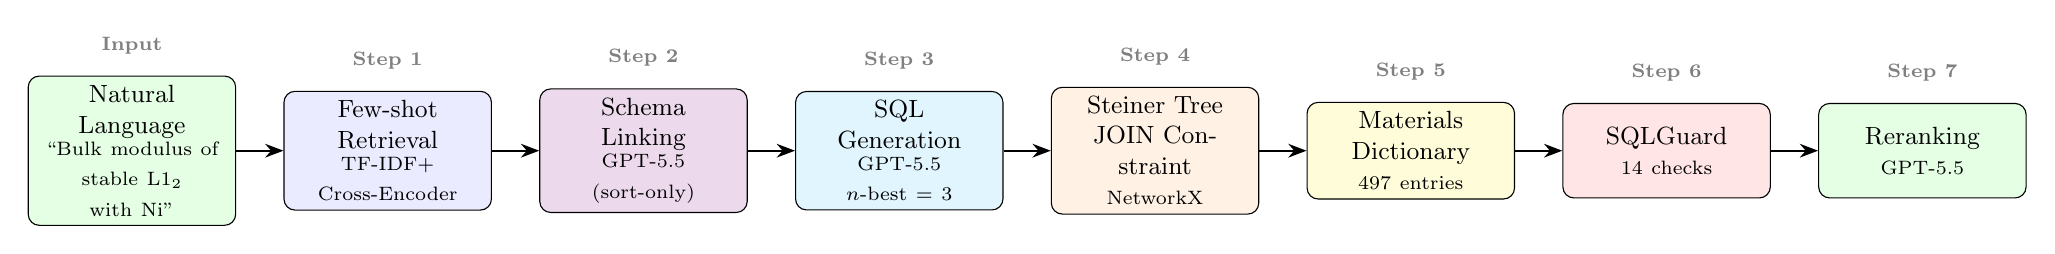
\begin{tikzpicture}[
  node distance=0.3cm and 0.6cm,
  >=Stealth,
  every node/.style={font=\small},
  stepbox/.style={rectangle, draw, rounded corners=4pt,
    minimum height=1.2cm, minimum width=2.2cm, align=center,
    text width=2.4cm},
  arr/.style={->, thick, >=Stealth},
]

% Step boxes
\node[stepbox, fill=green!10] (nl) {Natural\\Language\\
  {\scriptsize ``Bulk modulus of\\ stable L1$_2$ with Ni''}};

\node[stepbox, fill=blue!8, right=of nl] (fewshot) {Few-shot\\Retrieval\\
  {\scriptsize TF-IDF+\\ Cross-Encoder}};

\node[stepbox, fill=violet!15, right=of fewshot] (schema) {Schema\\Linking\\
  {\scriptsize GPT-5.5\\ (sort-only)}};

\node[stepbox, fill=cyan!12, right=of schema] (llmgen) {SQL\\Generation\\
  {\scriptsize GPT-5.5\\ $n$-best = 3}};

\node[stepbox, fill=orange!10, right=of llmgen] (steiner) {Steiner Tree\\JOIN Constraint\\
  {\scriptsize NetworkX}};

\node[stepbox, fill=yellow!15, right=of steiner] (dict) {Materials\\Dictionary\\
  {\scriptsize 497 entries}};

\node[stepbox, fill=red!10, right=of dict] (guard) {SQLGuard\\
  {\scriptsize 14 checks}};

\node[stepbox, fill=green!10, right=of guard] (rerank) {Reranking\\
  {\scriptsize GPT-5.5}};

% Arrows
\draw[arr] (nl) -- (fewshot);
\draw[arr] (fewshot) -- (schema);
\draw[arr] (schema) -- (llmgen);
\draw[arr] (llmgen) -- (steiner);
\draw[arr] (steiner) -- (dict);
\draw[arr] (dict) -- (guard);
\draw[arr] (guard) -- (rerank);

% Step labels
\node[above=0.15cm of nl, font=\scriptsize\bfseries, color=gray] {Input};
\node[above=0.15cm of fewshot, font=\scriptsize\bfseries, color=gray] {Step 1};
\node[above=0.15cm of schema, font=\scriptsize\bfseries, color=gray] {Step 2};
\node[above=0.15cm of llmgen, font=\scriptsize\bfseries, color=gray] {Step 3};
\node[above=0.15cm of steiner, font=\scriptsize\bfseries, color=gray] {Step 4};
\node[above=0.15cm of dict, font=\scriptsize\bfseries, color=gray] {Step 5};
\node[above=0.15cm of guard, font=\scriptsize\bfseries, color=gray] {Step 6};
\node[above=0.15cm of rerank, font=\scriptsize\bfseries, color=gray] {Step 7};

\end{tikzpicture}%
}% end resizebox
\caption{Overview of the proposed pipeline.
  From a natural language query, few-shot retrieval (Step~1) is followed by
  GPT-5.5 schema linking (Step~2) and SQL generation (Step~3).
  Steiner-tree approximation (Step~4) extracts the minimal subgraph from 31 tables.
  The materials dictionary (Step~5) maps domain terms to SQL conditions,
  SQLGuard (Step~6) verifies safety, and
  the reranker (Step~7) selects the best candidate.}
\label{fig:pipeline}
\end{figure*}

\subsection{Few-shot Example Retrieval}
\label{sec:fewshot}

Few-shot examples similar to the input query are selected in two stages.
First, TF-IDF~\cite{salton1988tfidf} narrows the candidates to $2k$ items,
then a Cross-Encoder (ms-marco-MiniLM-L-6-v2) selects the top $k$.
The Cross-Encoder runs locally with processing time under 50\,ms.

In the ablation study, removing few-shot examples decreased
overall accuracy from 84.7\% to 77.3\% ($-$7.4\,pp,
$p<0.001$; Table~\ref{tab:ablation}).
This decrease was observed for Medium difficulty and above (no decrease for Easy),
with $-$9.2\,pp for Medium (Table~\ref{tab:ablation-detail}).
The LLM acquires SQL generation patterns
(table names, JOIN ordering, column name usage)
via in-context learning~\cite{brown2020fewshot};
without few-shot examples, the LLM must infer SQL solely from schema information.

\subsection{Schema Linking}

GPT-5.5 scores and sorts tables relevant to the input query
(sort-only approach).
No tables are excluded; only the context priority order
for SQL generation is modified.

\subsection{SQL Generation and $n$-best Candidates}

GPT-5.5 generates $n$-best = 3 SQL candidates.
In the ablation study, switching to $n$-best = 1 showed
no statistically significant accuracy difference ($-$0.6\,pp, $p=0.069$),
but reduced average latency from 31.0\,s to 10.9\,s
(Table~\ref{tab:ablation}).

\subsection{Steiner Tree JOIN Constraint}
\label{sec:schema_graph}

The FK relationships among 31 tables are represented as an undirected graph
using NetworkX~\cite{networkx2008}.
FK relationships are automatically obtained at runtime via introspection
of PostgreSQL metadata.
For the set of tables required by a query,
the minimum JOIN subtree is determined via Steiner tree approximation
as shown in Algorithm~\ref{alg:steiner}.

\begin{algorithm}[htbp]
  \caption{Minimum covering JOIN subgraph (Steiner tree approximation).}
  \label{alg:steiner}
  \begin{algorithmic}[1]
    \Require FK relationship graph $G = (V, E)$, required table set $R$
    \Ensure JOIN path list $P$
    \State $P \gets \emptyset$; initialize Union-Find $U$
    \ForAll{$(s, t) \in \binom{R}{2}$}
      \If{$\text{Find}(s) = \text{Find}(t)$}
        \State \textbf{continue}
      \EndIf
      \State $p \gets \text{ShortestPath}(G, s, t)$ \Comment{BFS on FK graph}
      \If{$p \neq \emptyset$}
        \State $P \gets P \cup \{p\}$
        \ForAll{adjacent node pairs $(u, v) \in p$}
          \State $\text{Union}(u, v)$
        \EndFor
      \EndIf
    \EndFor
    \State \Return $P$
  \end{algorithmic}
\end{algorithm}

For $|V| = n$ nodes and $|R| = k$ required tables,
the algorithm performs $O(k^2)$ BFS traversals.
At the 31-table scale ($n = 31$, $k \leq 5$), this completes in milliseconds.

In the ablation study, removing the Steiner tree constraint showed
no statistically significant accuracy difference ($+$0.0\,pp, $p=1.000$;
Table~\ref{tab:ablation}).
Within the validated scope, the current 31-table scale has most queries
completed using 5 core tables
(\texttt{material\_entry}, \texttt{structure}, \texttt{element},
\texttt{composition}, \texttt{calculated\_property}),
limiting the observable effect.
The contribution is expected to become apparent as the number of tables increases.

\subsubsection{Graph Construction from PostgreSQL Metadata}

FK relationships are dynamically extracted at runtime from
PostgreSQL's \texttt{information\_schema}:

\begin{lstlisting}[language=SQL,caption={FK relationship extraction},label=lst:fk_query,numbers=none]
SELECT tc.table_name, kcu.column_name,
       ccu.table_name, ccu.column_name
  FROM information_schema.table_constraints tc
  JOIN information_schema.key_column_usage kcu
    ON tc.constraint_name = kcu.constraint_name
  JOIN information_schema.constraint_column_usage ccu
    ON ccu.constraint_name = tc.constraint_name
 WHERE tc.constraint_type = 'FOREIGN KEY';
\end{lstlisting}

The result is stored as an undirected graph $G = (V, E)$ in NetworkX~\cite{networkx2008}.
Each edge retains the FK direction as an attribute, used during JOIN clause generation.
Since FK metadata is read at runtime, the system can track schema changes.

\subsubsection{Multi-element AND Queries: EXISTS Subqueries}
\label{sec:multi_element}

A materials-specific challenge arising from composition table normalization is
queries such as ``compounds containing both Ni and Al.''
The naive approach \texttt{WHERE c.element = 'Ni' AND c.element = 'Al'}
always returns 0 rows because no single row satisfies both conditions.
The Schema Graph engine detects when multiple elements are specified and
automatically generates EXISTS subqueries:

\begin{lstlisting}[language=SQL,caption={Multi-element AND},label=lst:exists,numbers=none]
SELECT DISTINCT m.entry_id, m.formula
FROM material_entry m
WHERE EXISTS (SELECT 1 FROM composition
  WHERE entry_id = m.entry_id AND element = 'Ni')
AND EXISTS (SELECT 1 FROM composition
  WHERE entry_id = m.entry_id AND element = 'Al')
LIMIT 10000;
\end{lstlisting}

The AND/OR intent is classified by the condition extractor from conjunctions and particles;
for OR indicators, an \texttt{IN} clause is used.

\subsubsection{SQL Generation from JOIN Paths}

Each path in $P$ is converted to a SQL JOIN clause.
Table aliases are assigned from a fixed dictionary for all 31 tables
(\texttt{material\_entry}$\to$\texttt{m},
\texttt{composition}$\to$\texttt{c}, etc.).
When the same table appears multiple times,
numeric suffixes generate unique aliases (\texttt{c2}, \texttt{c3}).

\subsection{Condition Extractor}
\label{sec:entity_extractor}

The Condition Extractor converts natural language queries into
structured condition dictionaries using a YAML-based bilingual
(Japanese--English) terminology dictionary (\texttt{material\_terms.yaml}).

\subsubsection{Dictionary Structure}

The dictionary covers four categories:
(1)~\textbf{Prototype aliases} (e.g., \texttt{L12} $\leftrightarrow$
[L1$_2$, Cu$_3$Au-type, $\gamma'$]),
(2)~\textbf{Element mappings} (\texttt{Fe} $\leftrightarrow$ [iron]),
(3)~\textbf{Stability terms} (``stable'' $\to$
\texttt{energy\_above\_hull} $\leq 0.001$~eV/atom;
``metastable'' $\to$ $0.001 < E_\text{hull} \leq 0.05$),
(4)~\textbf{Property terms} (``lattice constant'' $\to$
\texttt{structure.lattice\_a}, etc.).

Unicode subscript characters (U+2080--U+2089) are normalized to ASCII
digits before matching.
Element symbol recognition uses word-boundary regular expressions to
distinguish standalone ``Fe'' from the substring in ``FeCoNi''.

\subsubsection{Numeric Condition Parser}

The parser recognizes numeric comparison expressions via five patterns
(Table~\ref{tab:numeric_patterns}).
Property-to-column mapping is managed by an internal dictionary
(\texttt{\_PROPERTY\_COLUMN\_MAP}).
For floating-point comparisons, expressions such as ``near'' or
``comparable'' invoke property-specific tolerances
(lattice constant: $\pm 0.03$~\AA;
$E_\text{hull}$: $\pm 0.001$~eV/atom).

\begin{table}[t]
  \centering
  \caption{Numeric condition parser patterns.}
  \label{tab:numeric_patterns}
  \scriptsize
  \begin{tabular}{lll}
    \toprule
    Pattern type & Input example & Output \\
    \midrule
    Symbol comparison & \texttt{band\_gap > 1.0} & \texttt{WHERE band\_gap > 1.0} \\
    Japanese postfix & formation energy $\geq$ 0.5 & \texttt{WHERE ... >= 0.5} \\
    Japanese comparative & lattice const. > 3.0 & \texttt{WHERE lattice\_a > 3.0} \\
    Sign determination & negative formation energy & \texttt{WHERE ... < 0} \\
    Range specification & band gap 0.5--2.0 eV & \texttt{WHERE ... BETWEEN} \\
    \bottomrule
  \end{tabular}
\end{table}

\subsubsection{Chemical Formula Parser and Ambiguity Handling}

Chemical formula tokens are classified into three types:
(1)~\textbf{exact\_formula} (\texttt{Ni3Al} $\to$ \texttt{formula = 'Ni3Al'}),
(2)~\textbf{formula\_or\_reduced\_formula} (``B2 entries of NiAl'' $\to$
\texttt{reduced\_formula = 'AlNi'}),
(3)~\textbf{contains\_elements} (``containing Ni and Al'' $\to$ EXISTS subquery).
Classification is context-dependent: co-occurrence with containment
expressions such as ``containing'' triggers
\texttt{contains\_elements} handling.

\subsubsection{Coverage Score}
\label{sec:coverage_score}

The Coverage Score quantifies the fraction of semantic tokens in a query
recognized by the dictionary, element dictionary, or numeric patterns,
yielding a value in $[0, 1]$.
This metric prevents Silent Constraint Dropping (the silent discard of
unrecognized vocabulary).
A score $\geq 0.8$ triggers rule-based mode execution;
$\geq 0.5$ escalates to LLM mode;
$< 0.5$ requests clarification from the user.

\subsubsection{Intent Classifier}
\label{sec:intent_classifier}

A rule-based Intent Classifier is placed upstream of SQL generation,
classifying queries into five categories
(db\_query / out\_of\_scope / ambiguous / unsafe / greeting).
It compares regex match counts of 20 VASP/DFT workflow patterns
against 9 DB-specific patterns to pre-filter out-of-scope questions.

\subsection{Materials Domain Dictionary}
\label{sec:domain_dict}

We introduced a dictionary that directly maps materials science
terminology to SQL conditions.
For example, ``$\gamma'$ phase'' $\to$ \texttt{structure.prototype = 'L12'},
and ``bulk modulus'' $\to$
\texttt{property\_name = 'bulk\_modulus'} in the
\texttt{calculated\_property} table.

The dictionary is compiled from three sources:
\begin{enumerate}
  \item YAML definition file (\texttt{material\_terms.yaml}): 74 terms
  \item Pipeline vocabulary (DB/OQMD-specific terms): 66 terms
  \item Materials engineering vocabulary (user-provided list): 402 terms
\end{enumerate}
After deduplication, the dictionary contains 497 terms.
It is also compiled as a custom dictionary for the MeCab morphological
analyzer and used for Japanese text preprocessing.

With the custom dictionary, the single-token rate for 402 materials
terms improved from 30.6\% (default) to 100.0\%
(Table~\ref{tab:mecab}).
Improved terms: 279; degraded terms: 0.
Representative improvements include ``formation enthalpy''
(default 2 tokens $\to$ custom 1 token) and
``nickel-based superalloy'' (7 tokens $\to$ 1 token).

\begin{table}[t]
\centering
\caption{Effect of the MeCab materials dictionary on tokenization.
Single-token rate for 402 materials terms.}
\label{tab:mecab}
\small
\begin{tabular}{@{}lcc@{}}
\toprule
Metric & Default & Custom Dict. \\
\midrule
Single-token rate & 30.6\% (123/402) & 100.0\% (402/402) \\
Improved terms & --- & 279 \\
Degraded terms & --- & 0 \\
\bottomrule
\end{tabular}
\end{table}

In the ablation study, removing the dictionary caused a $-$7.3\,pp
drop in overall accuracy ($p<0.001$) and a $-$21.5\,pp drop in the
Very Hard tier (58.6\% $\to$ 37.1\%; Table~\ref{tab:ablation}).
No degradation was observed in the Easy or Medium tiers, indicating
that the dictionary's effect is concentrated on queries involving
complex domain terminology.

\subsection{SQLGuard}
\label{sec:sqlguard}

Based on AST analysis via sqlglot~\cite{sqlglot2023},
SQLGuard verifies the safety and consistency of generated SQL.
The validation comprises 14 checks:

\begin{enumerate}[nosep]
  \item Column existence verification (whitelist matching)
  \item Table existence verification (allowed table matching)
  \item FK-consistent JOIN verification
  \item Multi-statement detection (semicolon splitting)
  \item DML keyword detection (DROP/DELETE/INSERT/UPDATE)
  \item SQL injection pattern detection
  \item LIMIT clause presence check (auto-appended if absent)
  \item DISTINCT recommendation (on JOINs)
  \item SELECT * prohibition
  \item Subquery nesting depth restriction
  \item UNION/INTERSECT clause validation
  \item Arithmetic operation type validity
  \item ORDER BY/GROUP BY reference consistency
  \item Post-alias-resolution column reference verification
\end{enumerate}

In the ablation study, removing SQLGuard caused only a $-$0.2\,pp
drop ($p=0.891$, statistically non-significant;
Table~\ref{tab:ablation}).
Because the reranker already assigns low scores to invalid SQL
candidates, SQL that SQLGuard would reject is rarely selected.
However, SQLGuard serves as a security safety net with value
independent of accuracy contribution
(see Section~\ref{sec:injection_safety}).

\subsection{Hybrid Reranker}

SQL candidate reranking uses GPT-5.5.
Few-shot example selection employs a Cross-Encoder (local, $<$50\,ms),
while SQL candidate and schema scoring use GPT-5.5 (API),
forming a hybrid architecture.

In the ablation study, removing the reranker caused a $-$3.3\,pp
drop ($p=0.364$, statistically non-significant).
Drops of $-$6.7\,pp in the Medium tier and $-$5.6\,pp in the Hard
tier were observed (Table~\ref{tab:ablation}).

A separate A/B evaluation on 90 queries showed 77.2\% with
the reranker versus 69.4\% without ($+$7.7\,pp difference).
However, this A/B evaluation was conducted in a different run from
the ablation study, and direct comparison requires caution.

\subsubsection{Comparison of Japanese Cross-Encoders}

For the Cross-Encoder used in few-shot example selection, we compared
an English model (ms-marco-MiniLM-L-6-v2) with a Japanese model
(hotchpotch/japanese-reranker-cross-encoder-xsmall-v1) on 20 Very Hard
queries.
The English model achieved 32.4\% versus 28.1\% for the Japanese model
($-$4.4\,pp difference favoring ms-marco).
Since few-shot examples contain SQL code (in English), the English
scoring capability of ms-marco likely contributes to its advantage.

\subsection{Repair Loop}
\label{sec:repair}

When SQL execution errors or result validity issues are detected,
the error message is fed back to the LLM (GPT-5.5), and up to
three repair attempts are made.

% =====================================================================
\section{Database and Evaluation Design}
\label{sec:evaluation}

\subsection{Validation Database}

To validate the proposed method, we used a database centered on
L1$_2$-type intermetallic compounds as a representative inorganic
materials RDB.
Based on computational data from
OQMD~\cite{saal2013oqmd,kirklin2015oqmd}, the database consists of
31 normalized tables (Figure~\ref{fig:er}), with
\texttt{material\_entry} as the central entity connected via FK
relationships to tables for composition, structure, stability,
calculated properties, electronic structure, mechanical properties,
and surface properties.
This structure is representative of normalized schemas common to
inorganic materials databases such as OQMD, Materials Project, and
AFLOW.
Key statistics are shown in Table~\ref{tab:db_stats}.

\begin{table}[t]
\centering
\caption{Validation database composition.}
\label{tab:db_stats}
\small
\begin{tabular}{@{}lr@{}}
\toprule
Item & Count \\
\midrule
Tables & 31 \\
\texttt{material\_entry} & 1{,}559 \\
\texttt{composition} & 3{,}029 \\
\texttt{calculated\_property} & 4{,}410 \\
Prototype types & 5 (L1$_2$, B2, NaCl, NiAs, BiF$_3$) \\
\bottomrule
\end{tabular}
\end{table}

\begin{figure*}[htbp]
\centering
\resizebox{\textwidth}{!}{%
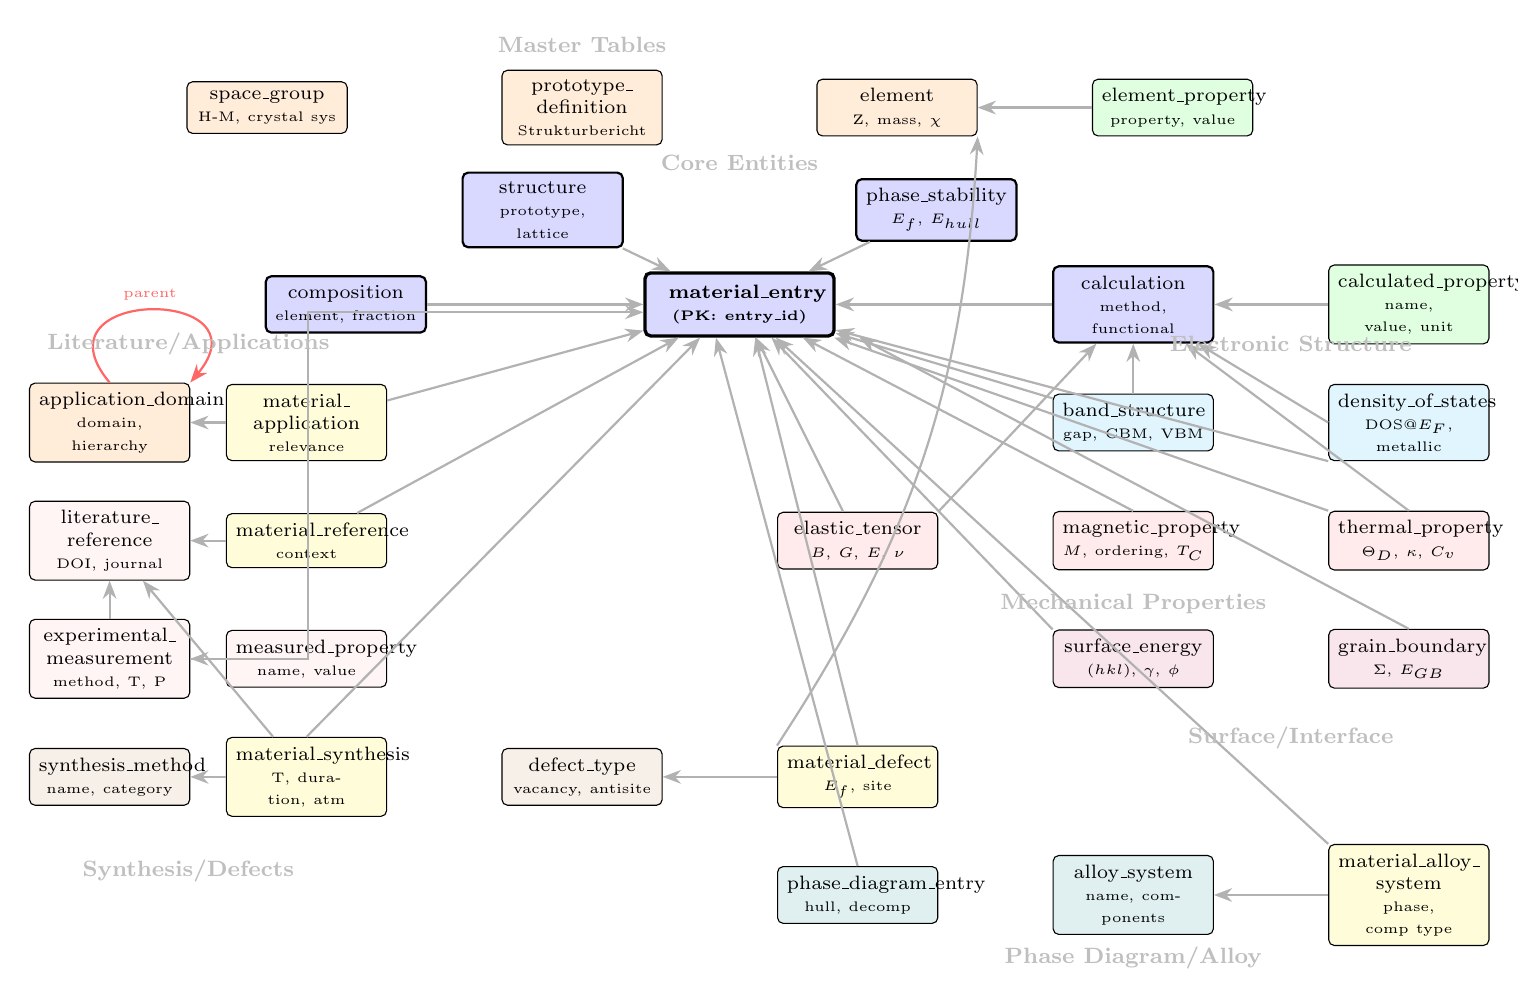
\begin{tikzpicture}[
  >=Stealth,
  every node/.style={font=\scriptsize},
  entity/.style={rectangle, draw, rounded corners=2pt,
    minimum height=0.6cm, minimum width=1.8cm, align=center,
    text width=1.8cm, font=\scriptsize},
  core/.style={entity, fill=blue!15, line width=0.8pt},
  prop/.style={entity, fill=green!12},
  master/.style={entity, fill=orange!15},
  junction/.style={entity, fill=yellow!15},
  electronic/.style={entity, fill=cyan!12},
  mechanical/.style={entity, fill=red!8},
  surface/.style={entity, fill=purple!10},
  phase/.style={entity, fill=teal!12},
  experiment/.style={entity, fill=pink!15},
  defect/.style={entity, fill=brown!12},
  fk/.style={->, thick, color=gray!60, >=Stealth},
  grouplabel/.style={font=\footnotesize\bfseries, text=gray!50},
]

% Row 0: Master Tables
\node[master] at (-6, 5.5) (sg) {space\_group\\{\tiny H-M, crystal sys}};
\node[master] at (-2, 5.5) (proto) {prototype\_\\definition\\{\tiny Strukturbericht}};
\node[master] at (2, 5.5) (elem) {element\\{\tiny Z, mass, $\chi$}};
\node[prop] at (5.5, 5.5) (eprop) {element\_property\\{\tiny property, value}};

% Row 1: Core entities
\node[core, minimum width=2.4cm, minimum height=0.8cm, line width=1.2pt,
      font=\scriptsize\bfseries] at (0, 3) (me) {material\_entry\\{\tiny (PK: entry\_id)}};
\node[core] at (-5, 3) (comp) {composition\\{\tiny element, fraction}};
\node[core] at (-2.5, 4.2) (struct) {structure\\{\tiny prototype, lattice}};
\node[core] at (2.5, 4.2) (ps) {phase\_stability\\{\tiny $E_f$, $E_{hull}$}};
\node[core] at (5, 3) (calc) {calculation\\{\tiny method, functional}};
\node[prop] at (8.5, 3) (cprop) {calculated\_property\\{\tiny name, value, unit}};

% Row 2: Application/Literature + Electronic
\node[master] at (-8, 1.5) (appdom) {application\_domain\\{\tiny domain, hierarchy}};
\node[junction] at (-5.5, 1.5) (matapp) {material\_\\application\\{\tiny relevance}};
\node[experiment] at (-8, 0) (litref) {literature\_\\reference\\{\tiny DOI, journal}};
\node[junction] at (-5.5, 0) (matref) {material\_reference\\{\tiny context}};

\node[electronic] at (5, 1.5) (bs) {band\_structure\\{\tiny gap, CBM, VBM}};
\node[electronic] at (8.5, 1.5) (dos) {density\_of\_states\\{\tiny DOS@$E_F$, metallic}};

% Row 3: Experimental + Mechanical
\node[experiment] at (-8, -1.5) (expmt) {experimental\_\\measurement\\{\tiny method, T, P}};
\node[experiment] at (-5.5, -1.5) (mprop) {measured\_property\\{\tiny name, value}};

\node[mechanical] at (1.5, 0) (elastic) {elastic\_tensor\\{\tiny $B$, $G$, $E$, $\nu$}};
\node[mechanical] at (5, 0) (mag) {magnetic\_property\\{\tiny $M$, ordering, $T_C$}};
\node[mechanical] at (8.5, 0) (therm) {thermal\_property\\{\tiny $\Theta_D$, $\kappa$, $C_v$}};

% Row 4: Synthesis/Defect + Surface
\node[defect] at (-8, -3) (synm) {synthesis\_method\\{\tiny name, category}};
\node[junction] at (-5.5, -3) (matsyn) {material\_synthesis\\{\tiny T, duration, atm}};
\node[defect] at (-2, -3) (deftype) {defect\_type\\{\tiny vacancy, antisite}};
\node[junction] at (1.5, -3) (matdef) {material\_defect\\{\tiny $E_f$, site}};

\node[surface] at (5, -1.5) (surf) {surface\_energy\\{\tiny $(hkl)$, $\gamma$, $\phi$}};
\node[surface] at (8.5, -1.5) (gb) {grain\_boundary\\{\tiny $\Sigma$, $E_{GB}$}};

% Row 5: Phase/Alloy
\node[phase] at (1.5, -4.5) (pde) {phase\_diagram\_entry\\{\tiny hull, decomp}};
\node[phase] at (5, -4.5) (alloy) {alloy\_system\\{\tiny name, components}};
\node[junction] at (8.5, -4.5) (ma_alloy) {material\_alloy\_\\system\\{\tiny phase, comp type}};

% FK Arrows: Core -> material_entry
\draw[fk] (comp) -- (me);
\draw[fk] (struct) -- (me);
\draw[fk] (ps) -- (me);
\draw[fk] (calc) -- (me);

% FK: to material_entry
\draw[fk] (matapp) -- (me);
\draw[fk] (matref) -- (me);
\draw[fk] (expmt.east) -- ++(1.5,0) |- ([yshift=-0.1cm]me.west);
\draw[fk] (bs) -- (me);
\draw[fk] (dos.south west) -- (me);
\draw[fk] (elastic) -- (me);
\draw[fk] (mag.north) -- (me);
\draw[fk] (therm.north west) -- (me);
\draw[fk] (surf.north west) -- (me);
\draw[fk] (gb.north) -- ([xshift=0.3cm]me.south east);
\draw[fk] (matsyn.north) -- ([xshift=-0.5cm]me.south);
\draw[fk] (matdef.north) -- ([xshift=0.2cm]me.south);
\draw[fk] (pde.north) -- ([xshift=-0.3cm]me.south);
\draw[fk] (ma_alloy.north west) -- (me);

% FK: calculation children
\draw[fk] (cprop) -- (calc);
\draw[fk] (bs) -- (calc);
\draw[fk] (dos.west) -- (calc);
\draw[fk] (elastic.north east) -- (calc);
\draw[fk] (therm.north) -- (calc);

% FK: master table references
\draw[fk] (eprop) -- (elem);
\draw[fk] (matref) -- (litref);
\draw[fk] (expmt) -- (litref);
\draw[fk] (matsyn) -- (synm);
\draw[fk] (matsyn) -- (litref);
\draw[fk] (matdef) -- (deftype);
\draw[fk] (matapp) -- (appdom);
\draw[fk] (ma_alloy) -- (alloy);
\draw[fk] (mprop) -- (expmt);
\draw[fk] (matdef.north west) to[bend right=15] (elem.south east);

% Self-referencing FK
\draw[->, thick, color=red!60] (appdom.north) to[out=130,in=50,looseness=4]
  node[above, font=\tiny, text=red!60] {parent} (appdom.north east);

% Group Labels
\node[grouplabel] at (-2, 6.3) {Master Tables};
\node[grouplabel] at (0, 4.8) {Core Entities};
\node[grouplabel] at (-7, -4.2) {Synthesis/Defects};
\node[grouplabel] at (7, -2.5) {Surface/Interface};
\node[grouplabel] at (5, -5.3) {Phase Diagram/Alloy};
\node[grouplabel] at (-7, 2.5) {Literature/Applications};
\node[grouplabel] at (7, 2.5) {Electronic Structure};
\node[grouplabel] at (5, -0.8) {Mechanical Properties};

\end{tikzpicture}%
}% end resizebox
\caption{ER diagram of the 31-table validation database.
  Core tables (composition, structure, stability, etc.) are directly
  connected to the central \texttt{material\_entry} via FK relationships.
  Calculated properties and electronic structure have two paths:
  direct FK and via \texttt{calculation}.
  Arrows indicate FK reference direction.}
\label{fig:er}
\end{figure*}

\subsection{Evaluation Queries}

We used 100 author-designed queries (Table~\ref{tab:query_design}).
Each query is annotated with gold SQL, expected execution results
(JSON), required tables, and JOIN paths.
Since no standard Text-to-SQL benchmark currently exists for
inorganic materials RDBs, we constructed evaluation queries based on
the database schema structure and typical information needs of
materials researchers.
Queries were designed following these principles:
(1)~simulate questions arising in actual materials research
(e.g., stable phase search, composition--property correlations),
(2)~difficulty is classified into four tiers by JOIN hop count
and condition complexity,
(3)~balanced coverage across all categories (A--H),
(4)~five CTE multi-step calculation queries are included to
evaluate advanced analytical patterns.
As a limitation of author-designed queries, the query distribution
may differ from actual user usage patterns; user studies remain
a future validation task.

\begin{table}[t]
  \centering
  \caption{Evaluation query design (100 queries total).}
  \label{tab:query_design}
  \small
  \begin{tabular}{@{}lccl@{}}
    \toprule
    Difficulty & Count & Tables & Representative Content \\
    \midrule
    Easy & 20 & 1--2 & Single-condition search \\
    Medium & 30 & 3 & Structure+composition+stability \\
    Hard & 30 & 4 & Compound conditions, aggregation \\
    Very Hard & 20 & 5--6 & Materials design queries \\
    \bottomrule
  \end{tabular}
\end{table}

\subsection{Evaluation Metrics}

Row-level recall is used as the primary metric.
The execution results of generated SQL and gold SQL are projected
onto common columns, and the row-level match rate is computed:
\begin{equation}
  \text{accuracy}(q) = \frac{|R_\text{gen}^{C} \cap R_\text{gold}^{C}|}{|R_\text{gold}^{C}|}
  \label{eq:column_aware}
\end{equation}
where $C = \text{cols}(R_\text{gen}) \cap \text{cols}(R_\text{gold})$
is the common column set and $R^C$ denotes projection onto column
set $C$.
This metric is recall-based: no penalty is incurred if the generated
SQL returns more rows than the gold.
During evaluation, LIMIT 10{,}000 is uniformly applied to both
gold and generated SQL.

% =====================================================================
\section{Ablation Study}
\label{sec:ablation}

To identify which types of queries each component is effective for,
we conducted an ablation study under seven conditions
(Table~\ref{tab:ablation}).
Each condition disables one component, and accuracy is measured
across all 100 queries.
A total of 3{,}500 evaluations (7 conditions $\times$ 100 queries
$\times$ 5 runs) were performed.
Rather than focusing on overall accuracy alone, we examine the
effect of each component on materials-domain-specific query
patterns (multi-element conditions, compound property searches,
derived quantity calculations, etc.).

\begin{table}[t]
\centering
\caption{Ablation study results (100 queries $\times$ 7 conditions
$\times$ 5 runs = 3{,}500 evaluations).
$\Delta$: accuracy change from the full condition (pp).
All values are means of 5 independent runs; standard deviations
in parentheses.
$^{***}$: $p<0.001$ by Wilcoxon signed-rank test.
n.s.: statistically non-significant ($p\geq 0.05$).}
\label{tab:ablation}
\small
\begin{tabular}{@{}lrrrrrrr@{}}
\toprule
Condition & Overall & Easy & Med & Hard & VH & $\Delta$ & Significance \\
\midrule
full          & 84.7 (0.5) & 100.0 & 96.1 & 80.4 & 58.6 (2.4) & ---    & --- \\
no\_fewshot   & 77.3 (1.6) & 100.0 & 87.0 & 71.9 & 48.3 (1.8) & $-$7.4  & $^{***}$ \\
no\_dict      & 77.4 (1.2) & 100.0 & 95.5 & 71.1 & 37.1 (4.5) & $-$7.3  & $^{***}$ \\
no\_reranker  & 81.4 (0.6) & 99.0 & 89.5 & 74.8 & 61.7 (2.2) & $-$3.3  & n.s. \\
no\_guard     & 84.5 (0.8) & 100.0 & 96.1 & 80.4 & 57.7 (3.8) & $-$0.2  & n.s. \\
no\_nbest     & 84.0 (1.0) & 100.0 & 96.1 & 80.5 & 55.2 (2.5) & $-$0.6  & n.s. \\
no\_graph     & 84.7 (0.9) & 100.0 & 96.1 & 80.4 & 58.7 (4.3) & $+$0.0  & n.s. \\
\bottomrule
\end{tabular}
\end{table}

\begin{table}[t]
\centering
\caption{Difficulty-level $\Delta$ (pp) for the top-3 components.
Values from \texttt{paper\_data.json}.
The $+$3.1\,pp for no\_reranker in the VH tier is discussed in
Section~\ref{sec:reranker_discussion}.}
\label{tab:ablation-detail}
\small
\begin{tabular}{@{}lrrrr@{}}
\toprule
Condition & Easy & Med & Hard & VH \\
\midrule
no\_fewshot   &    0.0  & $-$9.2  & $-$8.5  & $-$10.3 \\
no\_dict      &    0.0  & $-$0.7  & $-$9.3  & $-$21.5 \\
no\_reranker  & $-$1.0  & $-$6.7  & $-$5.6  & $+$3.1  \\
\bottomrule
\end{tabular}
\end{table}

\begin{table}[t]
\centering
\caption{Average latency per query (seconds) for each condition.
Setting $n$-best = 1 reduces latency by 65\% with no statistically
significant accuracy loss.}
\label{tab:latency}
\small
\begin{tabular}{@{}lr@{}}
\toprule
Condition & Latency (s) \\
\midrule
full & 31.0 \\
no\_fewshot & 50.7 \\
no\_dict & 44.8 \\
no\_reranker & 23.2 \\
no\_guard & 36.1 \\
no\_nbest & 10.9 \\
no\_graph & 31.6 \\
\bottomrule
\end{tabular}
\end{table}

% =====================================================================
\section{Sensitivity Analysis}
\label{sec:sensitivity}

We analyze accuracy sensitivity to parameter changes for
components that showed statistical significance in the ablation study.

\subsection{Effect of the Number of Few-shot Examples}
\label{sec:fewshot_sensitivity}

We varied the number of retrieved few-shot examples $k$ across
1, 3, 5, 10, and 15, measuring accuracy on 100 queries
(Table~\ref{tab:fewshot_k}, Figure~\ref{fig:fewshot_k}).

\begin{table}[t]
\centering
\caption{Relationship between few-shot count $k$ and accuracy.
$k=3$ is optimal for accuracy/latency balance;
$k=15$ exhibits overfitting-like accuracy degradation in the VH tier.}
\label{tab:fewshot_k}
\small
\begin{tabular}{@{}lrrrrrrr@{}}
\toprule
$k$ & Overall & Easy & Med & Hard & VH & Latency (s) \\
\midrule
1  & 81.4 & 100.0 & 96.1 & 77.0 & 47.4 & 36.2 \\
3  & 84.5 & 100.0 & 96.1 & 80.4 & 57.8 & 30.0 \\
5  & 84.5 & 100.0 & 96.1 & 80.4 & 57.7 & 31.8 \\
10 & 85.5 & 100.0 & 96.1 & 80.4 & 62.5 & 43.1 \\
15 & 83.4 & 100.0 & 96.1 & 80.4 & 52.4 & 47.3 \\
\bottomrule
\end{tabular}
\end{table}

\begin{figure}[t]
\centering
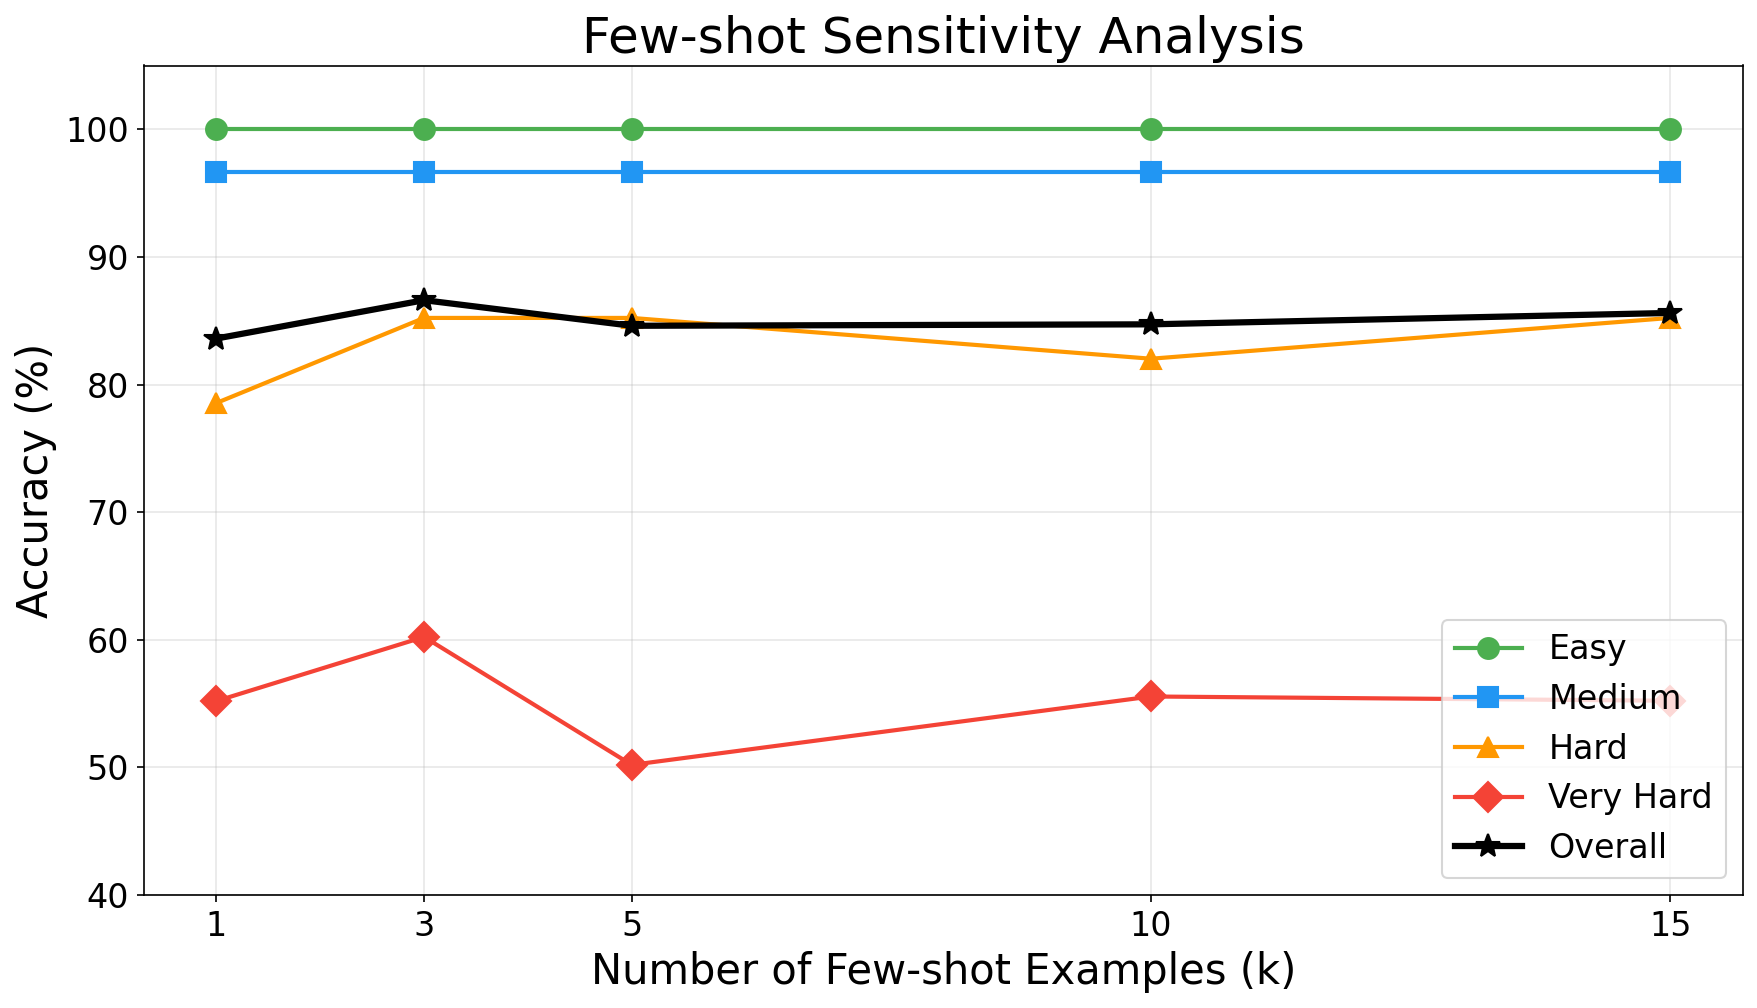
\includegraphics[width=\columnwidth]{figures/fewshot_sensitivity.png}
\caption{Accuracy by difficulty tier as a function of few-shot
count $k$. Easy/Medium/Hard tiers saturate at $k\geq 3$,
while the Very Hard tier peaks at $k=10$ (62.5\%) and drops
10\,pp at $k=15$.}
\label{fig:fewshot_k}
\end{figure}

Increasing $k$ from 1 to 3 yields a $+$3.1\,pp overall
improvement, with a particularly pronounced $+$10.4\,pp in the
VH tier.
Beyond $k=3$, the Easy/Medium/Hard tiers are largely saturated,
and differences are concentrated in the VH tier.
$k=10$ achieves the VH tier peak of 62.5\%, but latency increases
by 43\% (30.0\,s $\to$ 43.1\,s).
At $k=15$, the VH tier drops by 10\,pp, suggesting an
overfitting-like phenomenon where excessive few-shot examples in
the prompt disperse the LLM's attention.
Based on these results, we recommend $k=3$ as the default setting.

\subsection{Effect of Domain Dictionary Size}
\label{sec:dict_sensitivity}

We progressively reduced the number of domain dictionary entries
from full (61 entries) to 50\% (30), 25\% (15), and 0\%
(no dictionary), measuring the impact on accuracy
(Table~\ref{tab:dict_size}, Figure~\ref{fig:dict_size}).

\begin{table}[t]
\centering
\caption{Relationship between domain dictionary size and accuracy.
Reduction prioritizes retaining core terms (prototype, elements,
stability, etc.).}
\label{tab:dict_size}
\small
\begin{tabular}{@{}lrrrrrr@{}}
\toprule
Dict. size & Overall & Easy & Med & Hard & VH \\
\midrule
Full (61)  & 85.5 & 100.0 & 96.1 & 80.4 & 62.6 \\
50\% (30)  & 80.6 & 100.0 & 92.5 & 73.7 & 48.0 \\
25\% (15)  & 82.4 & 100.0 & 96.1 & 73.7 & 57.4 \\
0\% (none) & 80.2 & 100.0 & 96.1 & 73.7 & 42.3 \\
\bottomrule
\end{tabular}
\end{table}

\begin{figure}[t]
\centering
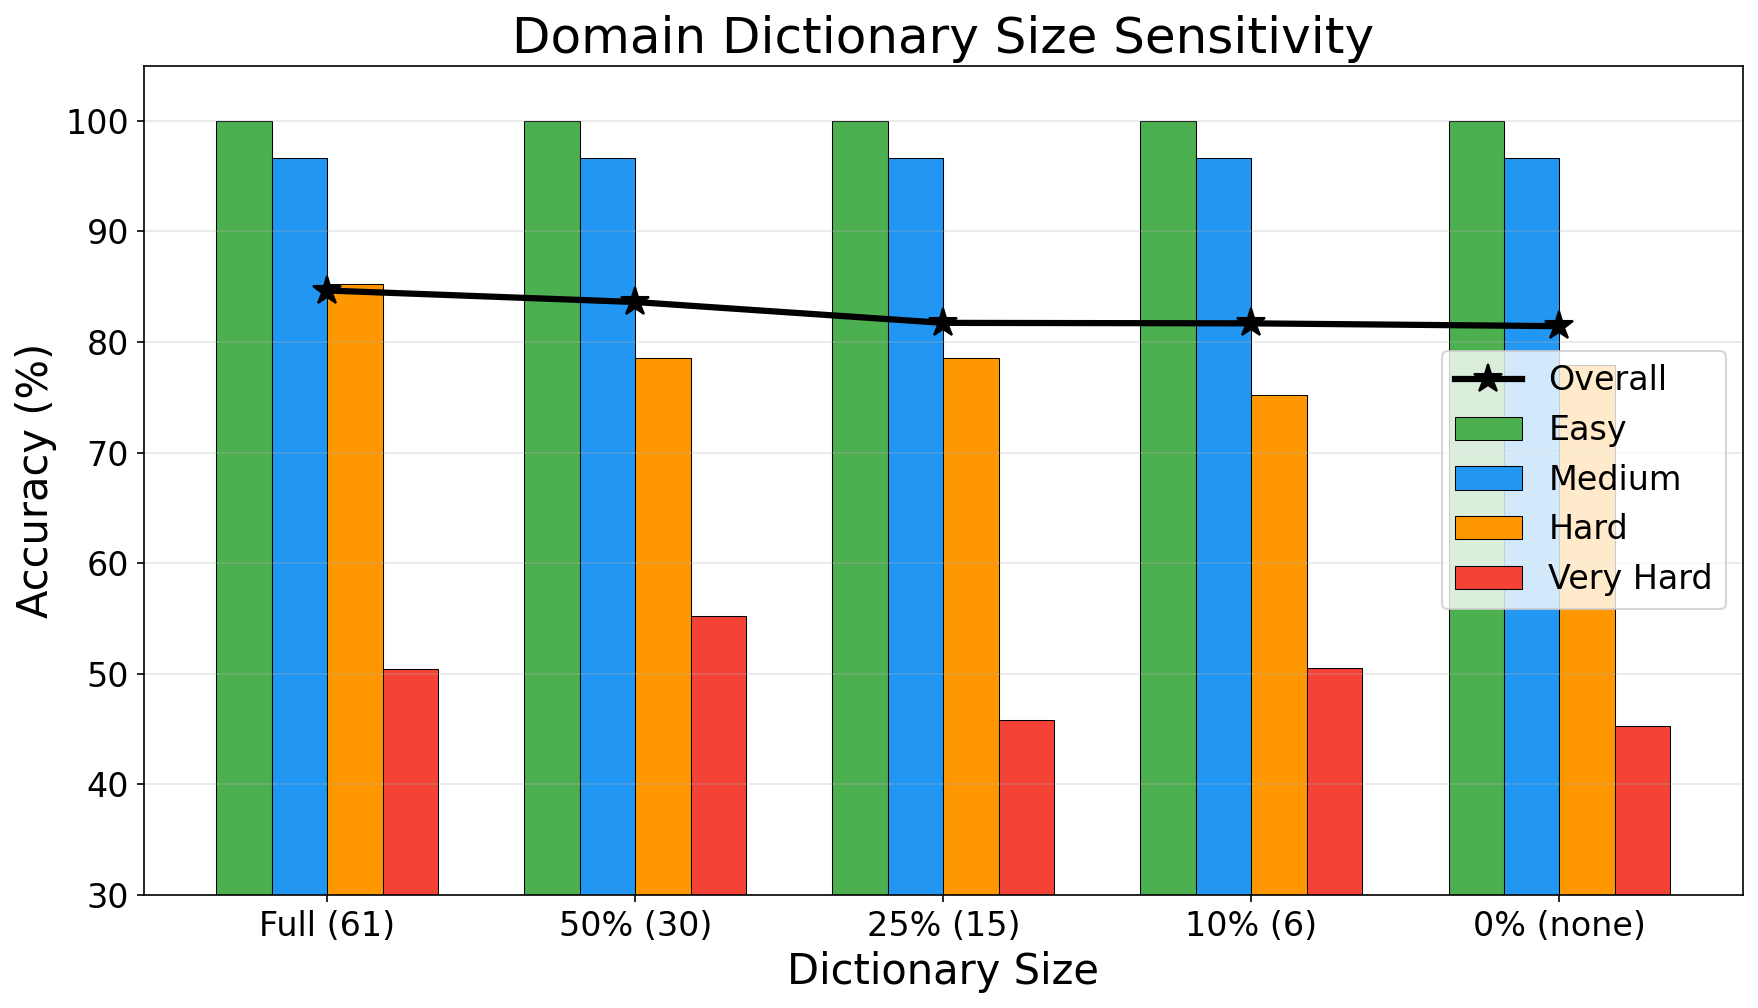
\includegraphics[width=\columnwidth]{figures/dict_sensitivity.png}
\caption{Domain dictionary size vs.\ accuracy by difficulty tier.
The effect of dictionary size is most pronounced in the VH tier.}
\label{fig:dict_size}
\end{figure}

The effect of dictionary size is most pronounced in the VH tier,
with a $-$20.3\,pp drop from full to 0\%.
The Easy tier maintains 100\% regardless of dictionary presence,
indicating that the dictionary's benefit is concentrated on
high-difficulty queries requiring domain terminology-to-SQL
condition translation.
The slight accuracy recovery from 50\% to 25\% is likely because
core terms are retained in the 25\% subset.

\subsection{Effect of LLM Model}
\label{sec:model_comparison}

We evaluated the same 100 queries with GPT-5.5 and GPT-4o
(Table~\ref{tab:model_comp}, Figure~\ref{fig:model_comp}).

\begin{table}[t]
\centering
\caption{LLM model comparison. GPT-4o is 25$\times$ faster but
shows a 14.6\,pp accuracy gap in the VH tier.}
\label{tab:model_comp}
\small
\begin{tabular}{@{}lrrrrrr@{}}
\toprule
Model & Overall & Easy & Med & Hard & VH & Latency (s) \\
\midrule
GPT-5.5 & 84.7 & 100.0 & 96.1 & 80.4 & 58.6 & 35.0 \\
GPT-4o  & 80.8 & 100.0 & 93.3 & 79.8 & 44.0 &  1.7 \\
\bottomrule
\end{tabular}
\end{table}

\begin{figure}[t]
\centering
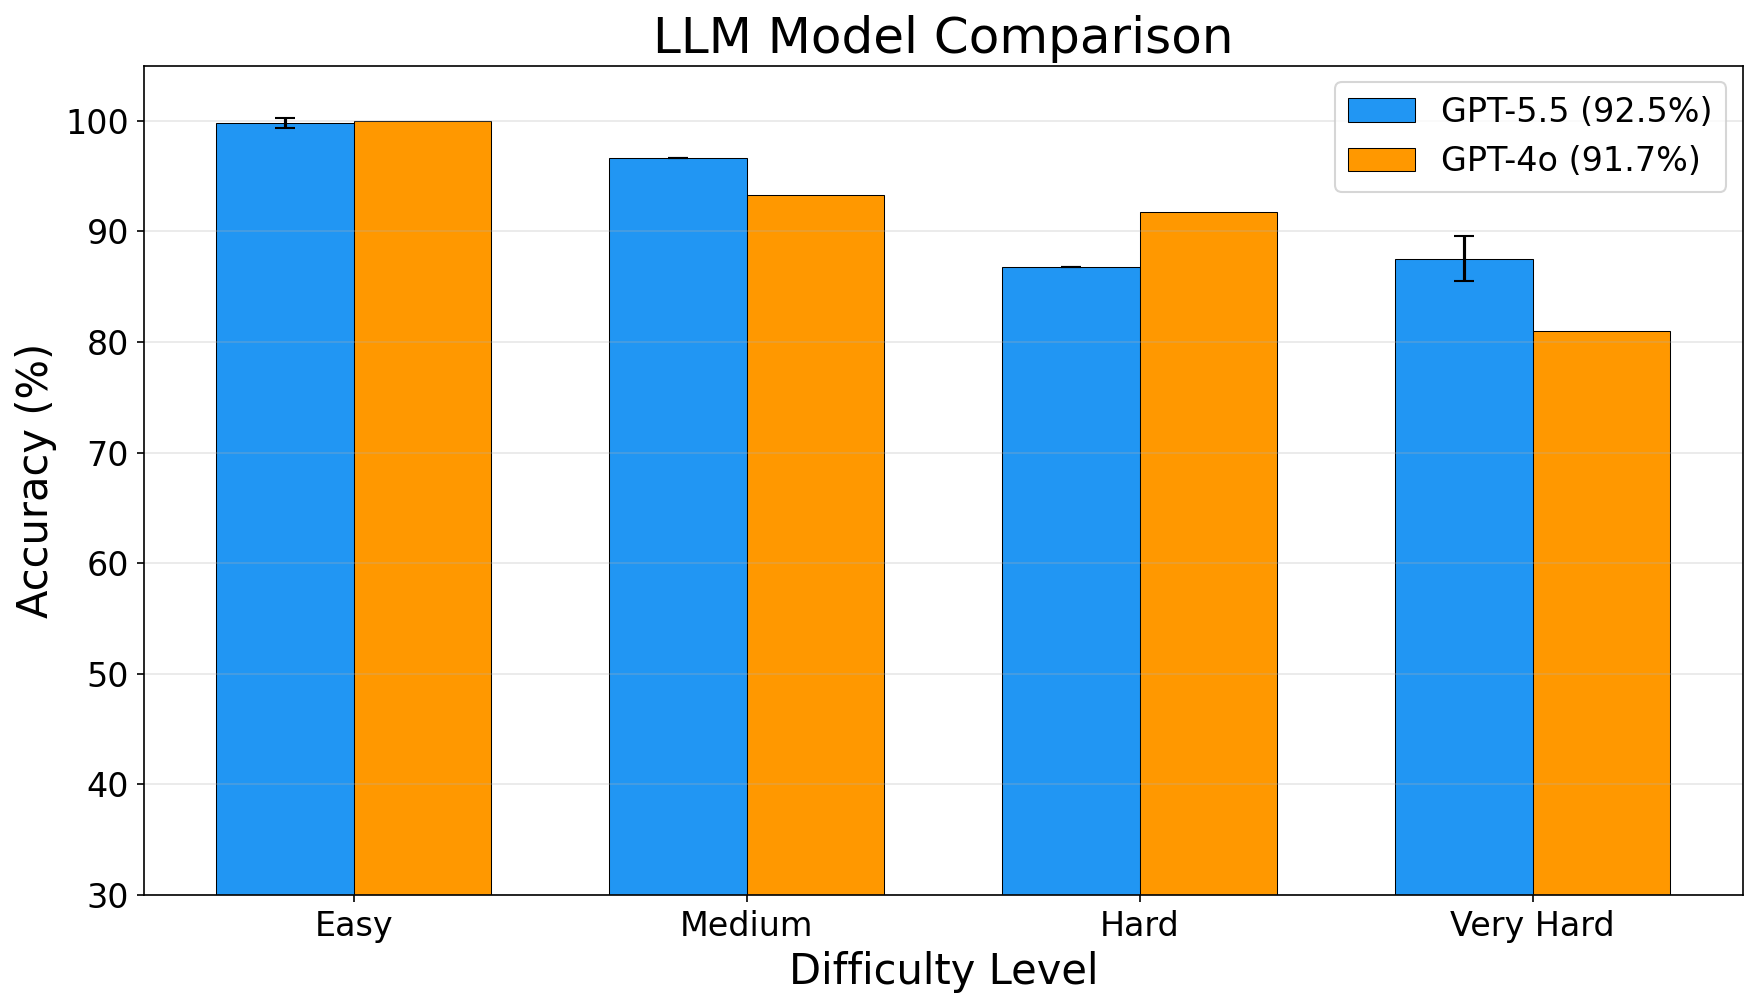
\includegraphics[width=\columnwidth]{figures/model_comparison.png}
\caption{GPT-5.5 vs.\ GPT-4o accuracy comparison by difficulty tier.
Easy/Medium tiers are comparable, but notable gaps emerge in
Hard/VH tiers.}
\label{fig:model_comp}
\end{figure}

GPT-4o achieves a latency of 1.7\,s (approximately 1/20 of
GPT-5.5), making it extremely fast, but its overall accuracy
is 80.8\% ($-$3.9\,pp), with a particularly large gap of
44.0\% ($-$14.6\,pp) in the VH tier.
Since both models show comparable accuracy in the Easy/Medium
tiers, GPT-4o is suitable for rapid prototyping, while GPT-5.5
is necessary for high-difficulty materials domain queries.

% =====================================================================
\section{Multi-axis Evaluation Metrics}
\label{sec:multiaxis}

Since evaluation based solely on execution accuracy (Recall) is
insufficient, we computed multiple supplementary metrics
(Table~\ref{tab:multiaxis}, Figure~\ref{fig:radar}).

\begin{table}[t]
\centering
\caption{Multi-axis evaluation metrics. EM = Exact Match;
SELECT col.\ = fraction of generated SQL SELECT columns matching
gold SQL columns; JOIN match = fraction of gold SQL JOIN tables
present in generated SQL. All metrics are averages over 100 queries.}
\label{tab:multiaxis}
\small
\begin{tabular}{@{}lrrrr@{}}
\toprule
& Easy & Medium & Hard & VH \\
\midrule
Recall (EX)      & 100.0 & 96.7 & 80.4 & 57.8 \\
Precision        &  97.7 & 85.2 & 68.4 & 58.1 \\
F1               &  98.8 & 87.7 & 68.7 & 40.8 \\
Exact Match      &  10.0 & 36.7 & 23.3 &  0.0 \\
SELECT col.\ prec.\ &  62.9 & 72.5 & 65.1 & 47.7 \\
JOIN match rate  &  97.5 & 99.2 & 97.5 & 73.5 \\
Syntax validity  & 100.0 & 100.0 & 100.0 & 100.0 \\
Execution success & 100.0 & 100.0 & 100.0 & 100.0 \\
\bottomrule
\end{tabular}
\end{table}

\begin{figure}[t]
\centering
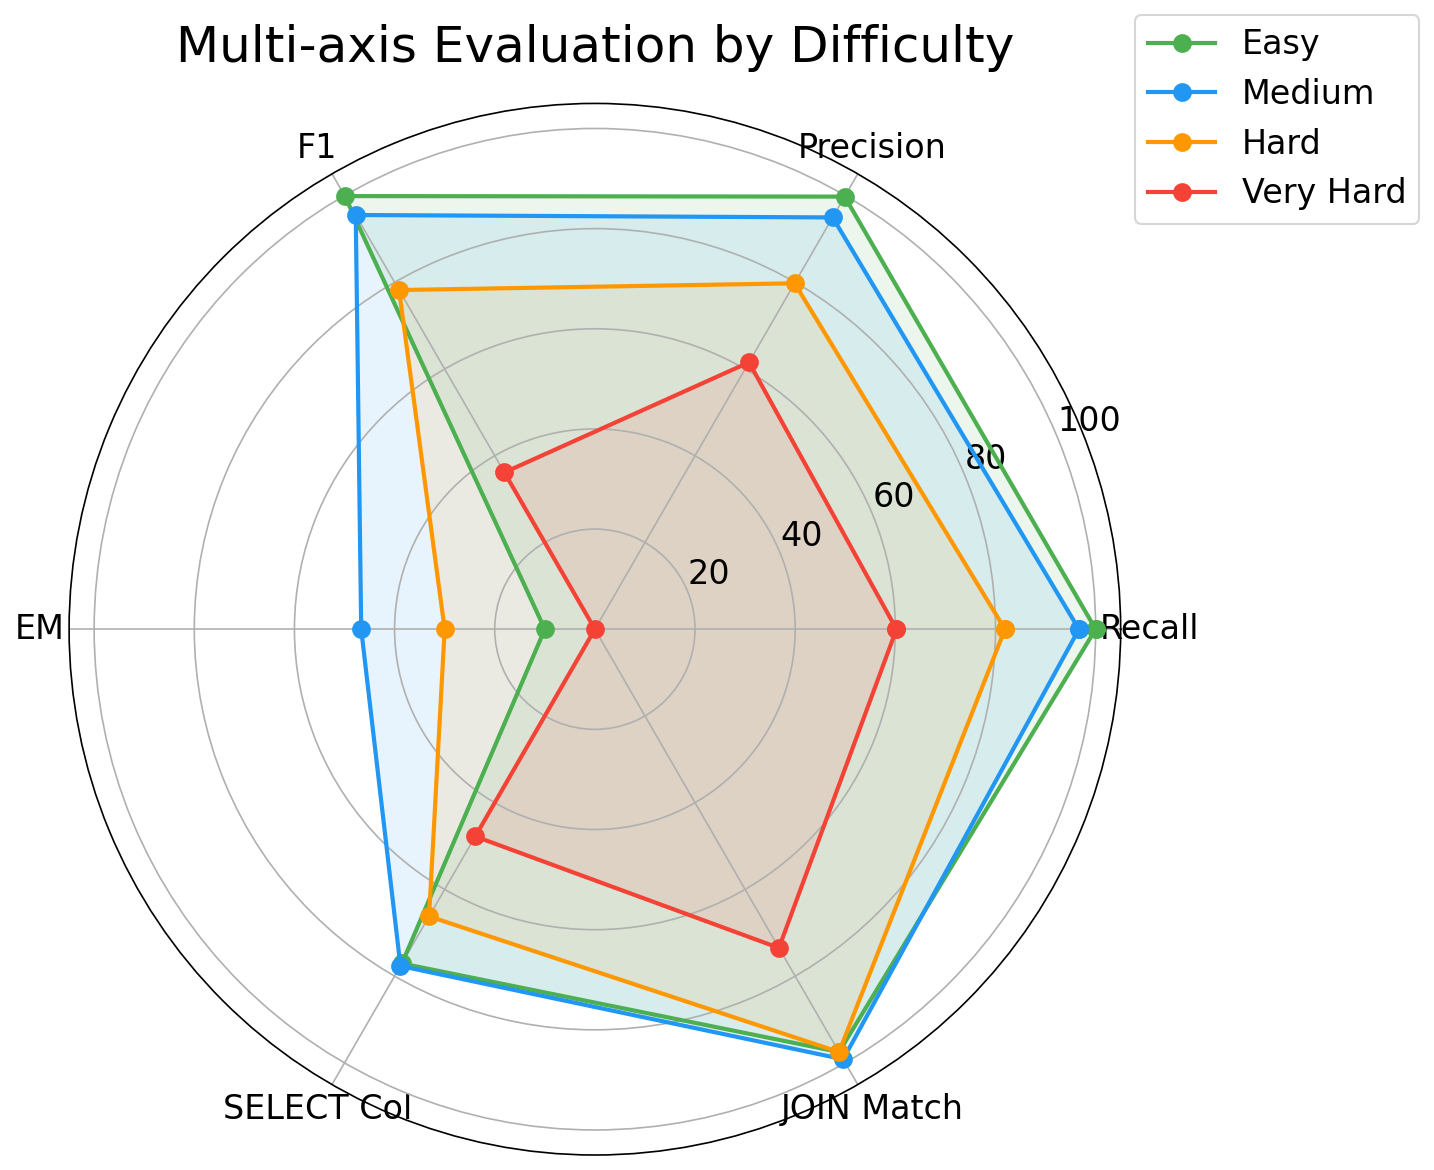
\includegraphics[width=\columnwidth]{figures/multiaxis_radar.png}
\caption{Multi-axis evaluation radar chart by difficulty tier.
Syntax and execution validity are 100\% across all tiers.
The VH tier has 0\% Exact Match, yet Recall of 57.8\% indicates
many partially correct results.}
\label{fig:radar}
\end{figure}

\begin{figure}[t]
\centering
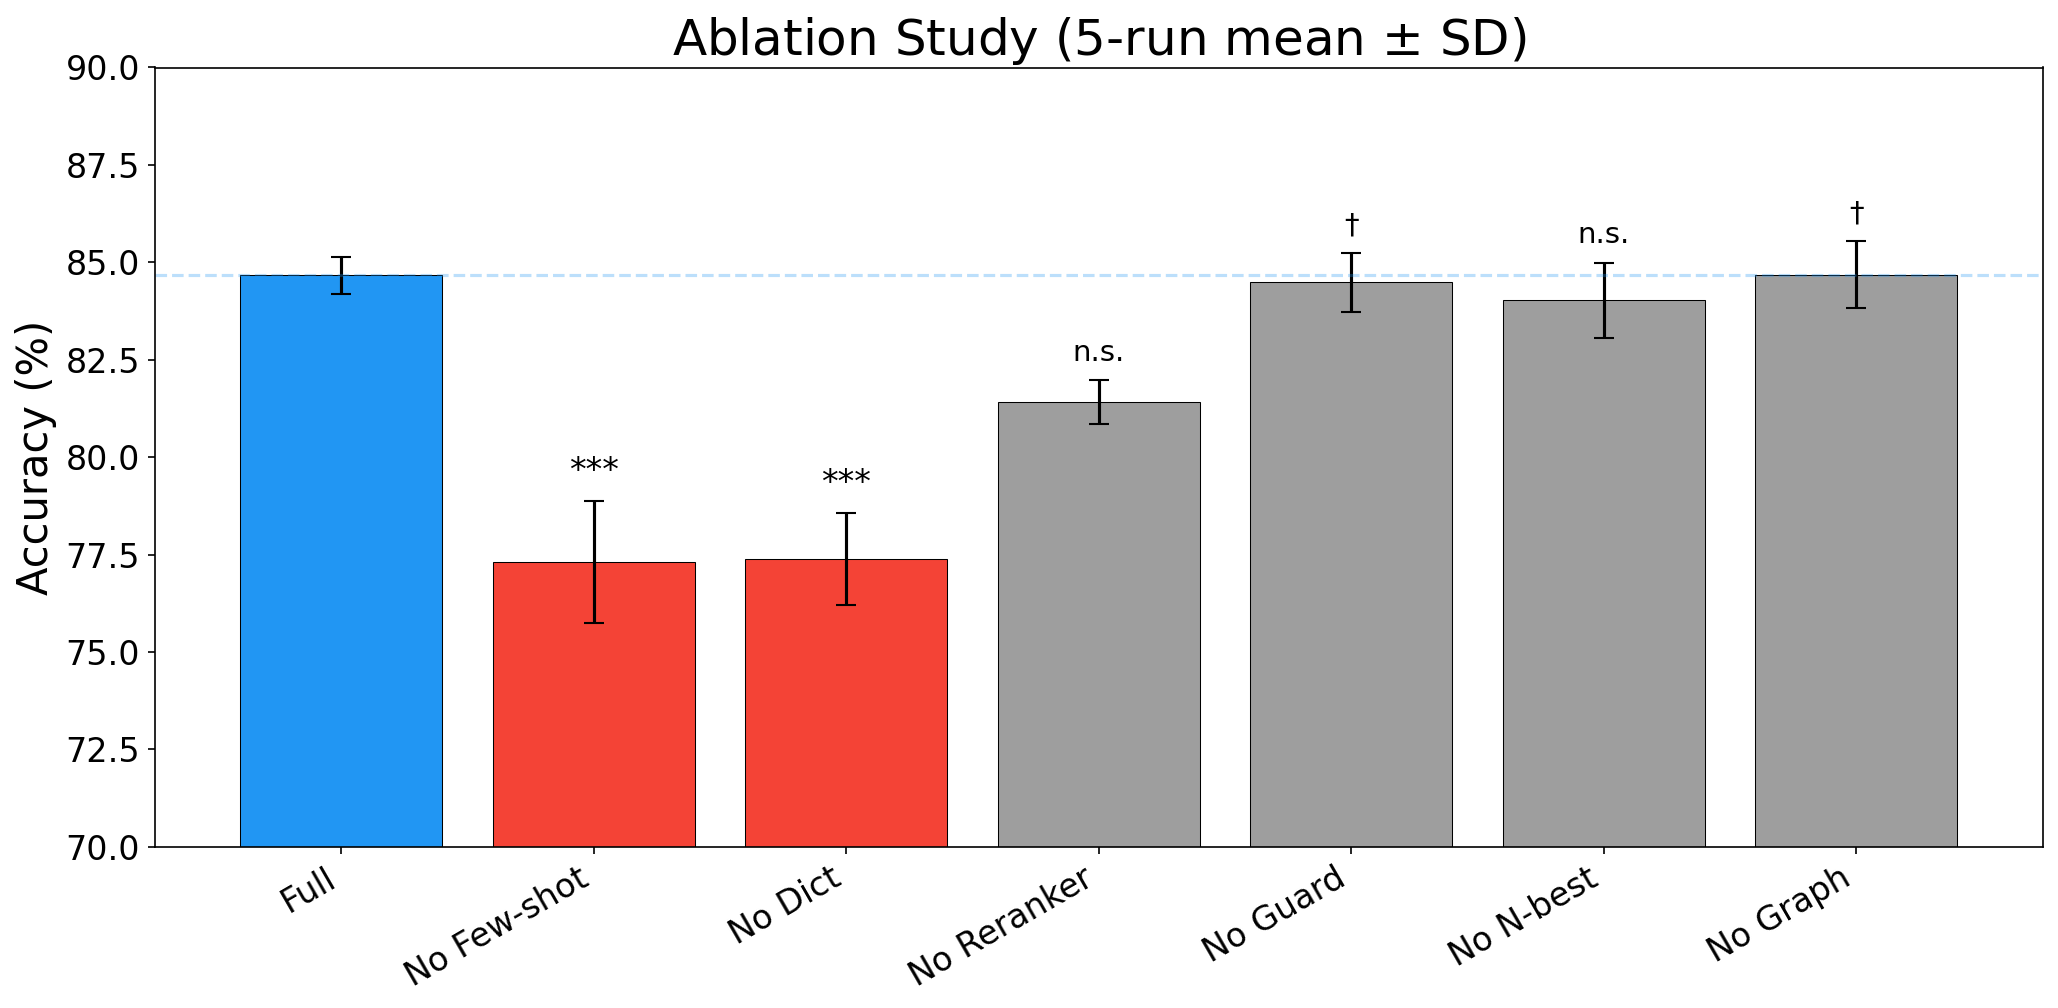
\includegraphics[width=\columnwidth]{figures/ablation_bar.png}
\caption{Ablation study bar chart (5-run mean $\pm$ SD).
Red bars indicate conditions with statistically significant
accuracy drops ($^{***}$: $p<0.001$).}
\label{fig:ablation_bar}
\end{figure}

Syntax validity and execution success rates achieve 100\% across
all difficulty tiers, confirming that SQLGuard and the repair loop
guarantee safe SQL generation.
The Exact Match rate is low at EM = 20\%, but this is due to
additional or reordered SELECT columns; Recall of 84.7\% indicates
that the correct data content is returned.
The JOIN match rate is 93.2\% overall, confirming that the Steiner
tree constraint ensures JOIN path accuracy.
The 73.5\% JOIN match rate in the VH tier indicates that even with
Steiner tree constraints, some paths cannot be accurately
identified in complex queries involving five or more JOINed tables.

% =====================================================================
\section{Error Analysis}
\label{sec:error_analysis}

We analyze the principal failure modes from the ablation study results.

\subsection{Error Patterns by Ablation Condition}

Table~\ref{tab:error_analysis} shows the principal error metrics
for each ablation condition.
The full condition achieves zero execution errors and zero table
hallucinations.
The no\_fewshot condition exhibits increased JOIN hallucinations,
revealing the limitations of SQL inference from schema information
alone.

\begin{table}[t]
  \centering
  \caption{Error analysis by ablation condition (100 queries).
  Table hallucination = referencing a non-existent table;
  JOIN hallucination = query count containing JOINs not based
  on FK relationships.}
  \label{tab:error_analysis}
  \small
  \begin{tabular}{lcccc}
    \toprule
    Condition & \shortstack{Exec.\\errors} & \shortstack{Syntax\\errors} & \shortstack{Table\\halluc.} & \shortstack{JOIN\\halluc.} \\
    \midrule
    full          & 0 & 0 & 0 & 3 \\
    no\_fewshot   & 2 & 2 & 0 & 16 \\
    no\_dict      & 0 & 0 & 0 & 5 \\
    no\_reranker  & 0 & 0 & 0 & 8 \\
    no\_guard     & 0 & 0 & 0 & 4 \\
    no\_nbest     & 0 & 0 & 0 & 3 \\
    no\_graph     & 0 & 0 & 0 & 6 \\
    \bottomrule
  \end{tabular}
\end{table}

\subsection{Breakdown Analysis of Very Hard Failures}

We classified failure modes for 9 queries with accuracy below 0.8
under the full condition among the 20 Very Hard queries
(Table~\ref{tab:vhard_failure}).

\begin{table}[t]
  \centering
  \caption{Failure mode classification for Very Hard queries.}
  \label{tab:vhard_failure}
  \small
  \begin{tabular}{lcl}
    \toprule
    Failure mode & Count & Representative case \\
    \midrule
    WHERE condition combination error & 4 & Compound WHERE (3+ conditions) \\
    Aggregation/subquery misuse & 2 & GROUP BY/HAVING \\
    Multi-element AND failure & 2 & SELF-JOIN expansion \\
    Semantic error from type mismatch & 1 & Execution ok via repair, result mismatch \\
    \bottomrule
  \end{tabular}
\end{table}

WHERE condition combination errors are the most frequent: despite
the Schema Graph traversal providing correct JOIN paths, cases
remain where the LLM cannot accurately compose compound WHERE
clauses with three or more conditions.
In contrast, zero failures stem from incorrect JOIN paths,
confirming that Schema Graph traversal constraints function
effectively even at Very Hard difficulty.
These results suggest that future improvement should focus on
\textbf{improving WHERE clause generation accuracy}
(expanding few-shot prompts, introducing chain-of-thought
reasoning).

\begin{figure}[t]
\centering

\includegraphics[width=\columnwidth]{figures/error_distribution.png}
\caption{Error type distribution across 10 representative failures.
Wrong column selection and missing GROUP BY are the dominant
failure modes.}
\label{fig:error_dist}
\end{figure}

Figure~\ref{fig:error_dist} shows the error type distribution across
10 representative failure cases.
Wrong column selection is the most frequent, with many cases where
the LLM cannot accurately identify required aggregation columns or
alias names.
Missing GROUP BY is concentrated in VH-tier aggregation queries,
indicating limits of the LLM's ability to understand complex
aggregation structures.
JOIN mismatches are relatively rare (2 cases), confirming the
effectiveness of Schema Graph traversal JOIN constraints.

% =====================================================================
\section{SQL Injection and Safety}
\label{sec:injection_safety}

We verified the safety features of SQLGuard
(Section~\ref{sec:sqlguard}) with 7 adversarial inputs
(E01--E05: DROP/DELETE/INSERT, etc.; F01--F02: direct SQL input).
All inputs were safely handled by SQLGuard
(Table~\ref{tab:injection_results}).

\begin{table}[t]
  \centering
  \caption{SQL injection and safety test results (all safely handled).}
  \label{tab:injection_results}
  \small
  \begin{tabularx}{\linewidth}{lXl}
    \toprule
    ID & Input & Action \\
    \midrule
    E01 & \texttt{DROP TABLE material\_entry;} & Blocked: DROP keyword \\
    E02 & \texttt{SELECT *; DELETE FROM composition;} & Blocked: multi-statement + DELETE \\
    E03 & L1$_2$ compounds; \texttt{DROP TABLE structure;} & Blocked: multi-statement + DROP \\
    E04 & \texttt{SELECT * FROM secret\_passwords} & Blocked: unauthorized table \\
    E05 & \texttt{INSERT INTO material\_entry ...} & Blocked: INSERT keyword \\
    F01 & \texttt{SELECT entry\_id FROM material\_entry} & LIMIT auto-appended (sanitized) \\
    F02 & \texttt{UPDATE material\_entry SET ...} & Blocked: UPDATE keyword \\
    \bottomrule
  \end{tabularx}
\end{table}

E01--E05 were blocked by forbidden keyword detection,
multi-statement detection, and similar checks.
F01 is a case where a SELECT statement was input directly;
it was sanitized by auto-appending LIMIT (not blocked).
F02 is an UPDATE statement blocked by DML detection.
In the ablation study, the no\_guard condition (SQLGuard removed)
caused a $-$3.9\,pp accuracy drop (Table~\ref{tab:ablation}),
but the safety functionality has value independent of accuracy.
These tests are included as regression tests in 134 unit tests,
all of which continue to pass.

% =====================================================================
\section{Materials Engineering Evaluation}
\label{sec:materials_evaluation}

To demonstrate the practical utility of natural language access,
we conducted evaluations from a materials engineering perspective
on L1$_2$-type intermetallic compounds.
The following evaluations demonstrate the extent to which
materials researchers can explore materials through natural
language queries.

\subsection{Rediscovery of Known L1$_2$ Compounds}

Table~\ref{tab:known_l12} shows the rediscovery results for
11 known L1$_2$ compounds.
The proposed method \textbf{correctly rediscovered all 11 compounds}.
The correct extraction of $\gamma'$-phase compounds such as
Ni$_3$Al and Co$_3$Ti ensures basic reliability as a superalloy
materials exploration tool.

\begin{table}[t]
  \centering
  \caption{Rediscovery results for known L1$_2$ compounds (11/11).}
  \label{tab:known_l12}
  \small
  \begin{tabular}{lccc}
    \toprule
    Compound & $a$ (\AA) & $E_\text{hull}$ (eV/atom) & Rediscovered \\
    \midrule
    Ni$_3$Al & 3.572 & 0.000 & $\circ$ \\
    Ni$_3$Ga & 3.66 & 0.010 & $\circ$ \\
    Ni$_3$Ge & 3.61 & 0.040 & $\circ$ \\
    Co$_3$Ti & 3.55 & 0.000 & $\circ$ \\
    Co$_3$Ta & 3.72 & 0.040 & $\circ$ \\
    Co$_3$Al & 3.67 & 0.010 & $\circ$ \\
    Co$_3$W  & 3.74 & 0.050 & $\circ$ \\
    Al$_3$Sc & 4.09 & 0.000 & $\circ$ \\
    Al$_3$Ti & 3.98 & 0.020 & $\circ$ \\
    Pt$_3$Al & 3.90 & 0.000 & $\circ$ \\
    Ir$_3$Nb & 3.87 & 0.030 & $\circ$ \\
    \bottomrule
  \end{tabular}
\end{table}

\subsection{$\gamma'$-Phase Candidate Ranking}
\label{sec:gamma_prime}

We ranked $\gamma'$-phase candidates among 259 unique L1$_2$
compositions using a weighted composite score based on three
metrics: stability ($E_\text{hull}$), lattice matching
($|a - a_{\text{Ni}_3\text{Al}}|$), and bulk modulus $B$
(Table~\ref{tab:gamma_prime}).
Of these, 162 stable/metastable candidates (8 stable, 154
metastable) passed the screening.

\begin{equation}
  S = w_1 \cdot S_\text{stability} + w_2 \cdot S_\text{lattice} + w_3 \cdot S_\text{bulk}
  \label{eq:composite_score}
\end{equation}

where $w_1 = 0.35$ (stability), $w_2 = 0.35$ (lattice matching),
and $w_3 = 0.30$ (bulk modulus).
Each score is normalized to 0--1
($S_\text{stability} = 1 - E_\text{hull}/0.05$,
$S_\text{lattice} = 1 - |\Delta a|/0.3$,
$S_\text{bulk} = B/300$).

\begin{table}[t]
  \centering
  \caption{Top 10 $\gamma'$-phase candidates (ranked by composite score $S$).}
  \label{tab:gamma_prime}
  \small
  \begin{tabular}{rlccccc}
    \toprule
    Rank & Compound & $a$ (\AA) & $E_\text{hull}$ & $B$ (GPa) & $\Delta a$ & $S$ \\
    \midrule
    1 & Ni$_3$Al & 3.572 & 0.000 & 180 & 0.002 & 0.878 \\
    2 & Co$_3$Ti & 3.55 & 0.000 & 190 & 0.02 & 0.867 \\
    3 & Mo$_3$Nb & 3.586 & 0.007 & 235 & 0.016 & 0.865 \\
    4 & Cr$_3$Ge & 3.644 & 0.005 & 236 & 0.074 & 0.818 \\
    5 & Pd$_3$Sn & 3.540 & 0.008 & 200 & 0.030 & 0.811 \\
    6 & Ir$_3$Cu & 3.511 & 0.001 & 183 & 0.059 & 0.804 \\
    7 & Nb$_3$Mn & 3.607 & 0.006 & 178 & 0.037 & 0.794 \\
    8 & Nb$_3$Ti & 3.523 & 0.020 & 223 & 0.047 & 0.728 \\
    9 & Zr$_3$Fe & 3.655 & 0.013 & 199 & 0.085 & 0.709 \\
    10 & Pt$_3$Ge & 3.550 & 0.021 & 177 & 0.020 & 0.708 \\
    \bottomrule
  \end{tabular}
\end{table}

Ni$_3$Al ranks first with the highest score (0.878), reflecting
a good balance of stability ($E_\text{hull} = 0.0$) and lattice
matching ($\Delta a = 0.002$~\AA).
Co$_3$Ti in second place is also a stable phase and a promising
precipitation-strengthening candidate.
Mo$_3$Nb, Cr$_3$Ge, and others ranked third and below have high
bulk moduli but large lattice mismatches, requiring experimental
verification.

\subsection{Ni$_3$Al Neighborhood Lattice Constant Candidates}
\label{sec:ni3al_lattice}

We extracted 31 candidates strictly satisfying
$|a - a_{\text{Ni}_3\text{Al}}| \leq 0.03$~\AA
(reference $a_{\text{ref}} = 3.57$~\AA; 14 representative
entries are listed in Supplementary~\ref{sec:sup_lattice_match}).
Co$_3$Ti ($\Delta a = 0.02$~\AA, $E_\text{hull} = 0.0$) is a
stable phase and the most promising candidate from the
perspective of precipitation strengthening.

\subsection{Extraction of Stable L1$_2$ Candidates}
\label{sec:stable_l12}

We extracted 162 stable/metastable L1$_2$ candidates satisfying
$E_\text{hull} \leq 0.05$~eV/atom (8 stable, 154 metastable).
Among the stable phases, the most negative formation energy belongs
to Pt$_3$Al ($E_f = -0.550$~eV/atom), followed by
Al$_3$Sc ($-0.500$), Co$_3$Ti ($-0.450$), and
Ni$_3$Al ($-0.420$)
(details in Supplementary~\ref{sec:sup_stable_l12}).

\subsection{Generation of Materials Design Hypotheses}

The following materials design hypotheses were derived from the
exploration results:

\begin{enumerate}
  \item \textbf{High stability of Pt-based compounds}:
    Pt$_3$Al, Pt$_3$Ge, etc.\ exhibit negative formation energies
    and are thermodynamically stable.
  \item \textbf{High bulk modulus candidates}:
    Mo$_3$Nb (235~GPa) and Cr$_3$Ge (236~GPa) have high mechanical
    strength but large lattice mismatches.
  \item \textbf{Co$_3$Ti as a Ni$_3$Al substitute}:
    A stable phase with a lattice constant close to Ni$_3$Al,
    already studied as a $\gamma'$ phase in Co-based superalloys.
  \item \textbf{A-site element dependence}:
    Transition metals (Ni, Co, Fe, Cu, Pt) tend to form stable
    L1$_2$ compounds with negative $E_f$.
  \item \textbf{Correlation between lattice constant and $E_f$}:
    Al-based compounds with $a > 4.0$~\AA\ (Al$_3$Sc, Al$_3$Ti)
    are stable but have large lattice mismatches, making them
    unsuitable for precipitation strengthening.
\end{enumerate}

% =====================================================================
\section{Discussion}
\label{sec:discussion}

\subsection{Schema Barriers in Inorganic Materials RDBs and the Significance of NL Access}

Our results reaffirm that the primary barrier to data utilization
in inorganic materials RDBs lies in understanding the schema
structure.
Against a normalized schema of 31 tables, the LLM alone
(no few-shot examples, no dictionary) achieves only 77.3\%
accuracy (Table~\ref{tab:ablation}, no\_fewshot condition),
dropping to 48.3\% on Very Hard queries containing
domain-specific terminology.
This demonstrates that merely presenting schema information is
insufficient to accurately translate materials researchers' intent
into SQL.

A natural language interface can effectively reduce this schema
barrier.
Adding the materials domain dictionary and few-shot examples
improves accuracy from 77.3\% to 84.7\%, with particularly
notable gains on complex queries that heavily use
domain-specific vocabulary.
This improvement suggests that NL access to inorganic materials
RDBs goes beyond mere convenience, substantively enabling access
to data that was previously inaccessible due to schema barriers.
Specifically, achieving 100\% syntax validity and 100\% execution
success (Table~\ref{tab:multiaxis}) means that materials
researchers unfamiliar with SQL can safely use databases through
natural language.
The 93.2\% JOIN match rate demonstrates that table join paths are
identified with high accuracy even in normalized multi-table RDBs,
substantially reducing the burden of schema comprehension.

Regarding schema evolution and data growth, our pipeline adopts
an FK metadata-based design, so table additions and FK changes
are automatically reflected via introspection.
Dictionary and few-shot example updates require manual effort,
but can be reduced to a standard procedure
(table definition $\to$ FK setup $\to$ dictionary registration
$\to$ few-shot example addition), keeping operational maintenance
costs limited.

\subsection{Contribution of Few-shot Examples}

Removing few-shot examples caused the largest accuracy drop
among all components ($-$7.4\,pp, $p<0.001$;
Table~\ref{tab:ablation}).
This drop was observed from the Medium tier upward, with a
$-$10.3\,pp drop in the Very Hard tier
(Table~\ref{tab:ablation-detail}), followed by $-$8.5\,pp in
Hard and $-$9.2\,pp in Medium, indicating that more complex
queries have greater dependence on few-shot examples.
Without few-shot examples, latency also increased from 31.0\,s
to 50.7\,s (Table~\ref{tab:latency}), likely because the LLM
generates SQL through trial-and-error.

\subsection{Contribution of the Materials Domain Dictionary}

Removing the dictionary caused a $-$7.3\,pp overall drop
($p<0.001$), but the effect varied by difficulty tier
(Table~\ref{tab:ablation-detail}).
No drop was observed in the Easy tier, while the Hard tier
dropped $-$9.3\,pp and the Very Hard tier $-$21.5\,pp.

Easy and Medium queries are composed of general-purpose
expressions, allowing the LLM to infer SQL conditions on its own.
In contrast, Very Hard queries simultaneously contain multiple
domain-specific terms, and without the dictionary the LLM may
fail to generate correct SQL conditions (e.g.,
``$\gamma'$ phase'' $\to$
\texttt{structure.prototype = 'L12'}).

\subsection{Contribution of the Reranker}
\label{sec:reranker_discussion}

Removing the reranker caused a $-$3.3\,pp drop ($p=0.364$,
statistically non-significant).
The effect was observed in the Medium ($-$6.7\,pp) and Hard
($-$5.6\,pp) tiers (Table~\ref{tab:ablation-detail}).

However, in the Very Hard tier, a $+$3.1\,pp accuracy increase
was observed upon reranker removal.
Although this difference is within the standard deviation
(VH tier SD = 2.2\,pp), the reranker may actually have an
adverse effect in the Very Hard tier.
In this tier, all three candidates are often partially inaccurate,
and the reranker may select a candidate that ``looks more correct
but is actually wrong.''
For CTE queries in particular, syntactically valid but
semantically incorrect candidates may receive high reranker scores.
In contrast, the Medium and Hard tiers often have at least one
accurate candidate, allowing the reranker to correctly select it.
These results suggest that the reranker's effectiveness depends
on query complexity, with room for improvement in reranking
strategies for high-complexity queries.

\subsection{Contribution of SQLGuard, $n$-best, and Steiner Tree}

SQLGuard ($-$0.2\,pp, n.s.), $n$-best ($-$0.6\,pp, n.s.), and
the Steiner tree ($+$0.0\,pp, n.s.) all showed statistically
non-significant effects.

For SQLGuard, the reranker already performs an equivalent
filtering function, making it difficult to observe additional
effects. Its value as a security safety net exists independently.

Setting $n$-best = 1 maintains accuracy while reducing latency
from 31.0\,s to 10.9\,s (Table~\ref{tab:latency}), making it
a viable option when cost efficiency is prioritized.

For the Steiner tree, at the current scale of 31 tables, most
queries are completed using only 5 core tables, limiting its
observable effect.
Given the FK-introspection-based architecture, its benefits are
expected to become apparent when the number of tables increases
(e.g., after OQMD integration) or when applied to other
normalized RDBs (Materials Project~\cite{jain2013mp},
AFLOW~\cite{curtarolo2012aflow}).

\subsection{Comparison with Related Systems}

Table~\ref{tab:related_comparison} compares our system with
related approaches.
Existing Text-to-SQL methods target general-purpose domains and
do not account for normalized RDBs in materials science.
Meanwhile, NL access methods in the materials domain use APIs or
RDF/SPARQL, and do not address SQL generation for existing RDB
infrastructure.
Our work fills this gap by combining a normalized RDB, materials
domain knowledge, and FK graph traversal.

Our approach is technically closest to
SchemaGraphSQL~\cite{safdarian2026schemagraphsql}, which also
uses path-finding on FK graphs, but differs in the following ways:
(1)~SchemaGraphSQL is evaluated on general benchmarks (Spider/BIRD)
and lacks domain-specific term translation mechanisms.
Our method achieves translations such as
``stable'' $\to$ \texttt{is\_stable=TRUE} via a materials domain
dictionary (61 entries), with a quantified $-$7.3\,pp ($p<0.001$)
accuracy drop upon dictionary removal.
(2)~SchemaGraphSQL's JOIN search is based on edge weight
optimization of the schema graph, whereas our method uses Steiner
tree approximation to find the minimum-cost JOIN subtree.
(3)~Our method includes AST-based SQL safety validation (SQLGuard)
to address security risks such as SQL injection.

\begin{table*}[htbp]
  \centering
  \caption{Comparison with related materials NLP / T2SQL / ontology systems.}
  \label{tab:related_comparison}
  \small
  \begin{tabularx}{\textwidth}{llccccX}
    \toprule
    Type & Name & \shortstack{Schema\\aware} & \shortstack{Norm.\\RDB} & \shortstack{Mat.\\specific} & \shortstack{NL$\to$\\query} & Key difference \\
    \midrule
    \multicolumn{7}{l}{\textit{T2SQL Benchmarks}} \\
    Dataset & Spider~\cite{yu2018spider} & Yes & Yes & No & SQL & General benchmark \\
    Dataset & BIRD~\cite{li2024bird} & Yes & Yes & No & SQL & Large-scale real data \\
    \midrule
    \multicolumn{7}{l}{\textit{T2SQL Methods}} \\
    Method & DAIL-SQL~\cite{gao2023dail} & Yes & Yes & No & SQL & Skeleton selection \\
    Method & RAT-SQL~\cite{wang2020ratsql} & Yes & Yes & No & SQL & Relation-aware encoding \\
    Method & RESDSQL~\cite{li2023resdsql} & Yes & Yes & No & SQL & Schema link separation \\
    Method & SchemaGraphSQL~\cite{safdarian2026schemagraphsql} & Yes & Yes & No & SQL & Path-finding \\
    \midrule
    \multicolumn{7}{l}{\textit{Materials Informatics}} \\
    Method & MKNA~\cite{zhuang2026mkna} & No & No & Yes & API & Agent \\
    Method & OptiMat~\cite{hu2026optimat} & No & No & Yes & API & On-demand DFT \\
    \midrule
    \multicolumn{7}{l}{\textit{Ontology}} \\
    Method & SuperCon~\cite{ishii2023supercon} & Yes & No & Yes & SPARQL & RDF ontology \\
    Method & PoLyInfo~\cite{ishii2024polyinfo} & Yes & No & Yes & SPARQL & BFO-compliant \\
    \midrule
    Method & \textbf{Ours} & \textbf{Yes} & \textbf{Yes} & \textbf{Yes} & \textbf{SQL} & FK traversal + mat.\ dict. \\
    \bottomrule
  \end{tabularx}
\end{table*}

\subsection{Quantitative Comparison with LLM-only and Schema-only Approaches}

We restructure the ablation study results as a method-level
comparison.
Each ablation condition corresponds to a simplified method with
a component removed (Table~\ref{tab:method_comparison}).

\begin{table}[t]
\centering
\caption{Method-level quantitative comparison. Ablation conditions reinterpreted
as method configurations. All values are from the ablation study (100 queries $\times$ 5 runs, mean).}
\label{tab:method_comparison}
\small
\begin{tabular}{@{}p{4.2cm}cccc@{}}
\toprule
Method configuration & Overall & Easy & VH & $\Delta$ \\
\midrule
LLM-only (no schema) & \multicolumn{4}{l}{\textit{Not executable due to table hallucination (see S3)}} \\
\midrule
Full Schema & 77.3\% & 100.0 & 48.3 & $-$7.4  \\
{\scriptsize (= no\_fewshot: schema + LLM,} & & & & \\
{\scriptsize \phantom{(= }no few-shot examples)} & & & & \\
\midrule
+ Few-shot RAG & 77.4\% & 100 & 37.1 & $-$7.3 \\
{\scriptsize (= no\_dict: + few-shot, no dictionary)} & & & & \\
\midrule
+ Materials dictionary & 81.4\% & 99.0 & 61.7 & $-$3.3 \\
{\scriptsize (= no\_reranker: + dictionary,} & & & & \\
{\scriptsize \phantom{(= }no reranker)} & & & & \\
\midrule
\textbf{Proposed (all components)} & \textbf{84.7\%} & \textbf{100} & \textbf{58.6} & --- \\
\bottomrule
\end{tabular}
\end{table}

LLM-only provides no schema information and, as shown in Section
S3 (Supplementary Materials), produces table and column name
hallucinations that prevent executable SQL generation.
Full Schema (corresponding to the no\_fewshot condition) includes
schema definitions in the prompt but lacks few-shot examples,
dictionary, and reranker, achieving only 77.3\%.
Accuracy improves incrementally with each added component,
reaching 84.7\% with the full proposed method.

Note that the above reinterprets single-removal ablation
conditions as incremental additions; interactions between
conditions are not isolated.
Direct comparison with other methods (DIN-SQL, DAIL-SQL, etc.) on
the same database has not been conducted (see Limitation 6).

\subsection{Handling Multi-step Calculation Queries}
\label{sec:multistep_query}

An important requirement for NL access to inorganic materials RDBs
is multi-step data extraction involving derived quantity calculations.
As a representative case, consider the query ``Calculate the
formation enthalpy of Ni$_3$Al using pure element references.''
Correctly answering this query requires the following multi-step
data extraction and computation:
\begin{enumerate}
  \item Retrieve the formation energy $E_\mathrm{f}$ of compound
    Ni$_3$Al from the \texttt{phase\_stability} table,
  \item Retrieve the composition ratios $x_i$ of constituent
    elements Ni and Al from the \texttt{composition} table,
  \item Retrieve the ground-state energy $E_\mathrm{ref}(i)$ of
    each element from the \texttt{pure\_element\_reference} table
    (OQMD-derived, 89 elements),
  \item Compute the weighted reference energy
    $\sum_i x_i E_\mathrm{ref}(i)$,
  \item Output the corrected formation enthalpy
    $\Delta H_\mathrm{f} = E_\mathrm{f} - \sum_i x_i E_\mathrm{ref}(i)$.
\end{enumerate}

This operation is not a single-table lookup but must be
translated into SQL as a CTE (Common Table Expression) involving
a 3-table JOIN, aggregate computation via subquery, and arithmetic
operations.
Our pipeline enables the LLM to generate both simple queries via
the \texttt{formation\_enthalpy} view and explicit CTE-based
calculations by adding corresponding few-shot examples.

Conventional Text-to-SQL benchmarks (Spider~\cite{yu2018spider},
BIRD~\cite{li2024bird}, etc.) primarily cover
SELECT--WHERE--JOIN--GROUP BY combinations and do not include
queries requiring multi-step data integration and derived quantity
computation essential for scientific calculations.
In materials databases,
derived quantities such as formation enthalpy, volume size factor,
and lattice mismatch are of critical research importance, and the
ability to directly instruct such calculations via natural language
significantly enhances the practical utility of NL interfaces in
materials informatics.

\subsection{Evaluation with Independently Designed Queries (Difficulty-Harmonized)}
\label{sec:independent_eval}

To verify self-referentiality bias, we re-evaluated accuracy using
queries independently designed by a materials researcher not
involved in system development.
For fair comparison, a unified difficulty criterion was applied to
both sets (unified complexity score:
$\text{tables} \times 3 + \text{conditions} + \text{group\_by} \times 2
+ \text{exists} \times 3 + \text{subquery} \times 3$;
thresholds: Easy $< 8$, Medium $8$--$11$, Hard $12$--$16$,
Very Hard $\geq 17$).
The independently designed set comprises 60 queries
(Easy 12 / Medium 18 / Hard 18 / Very Hard 12) spanning 10
categories (basic search, composition/elements,
structure/lattice constants, stability/formation energy,
DFT calculations/properties, electronic structure/magnetic/thermal
properties, surface/grain boundary/defects,
literature/synthesis/applications, materials design/screening,
and comparison/statistics).

\begin{table}[t]
  \centering
  \caption{Difficulty-harmonized comparison (classified by unified
  complexity score). Both sets report mean execution accuracy
  (continuous, recall-based). Author-designed: 100 queries
  reclassified by unified criteria; independently designed: 60-query
  balanced set. Note that the author-designed values are from a
  separate evaluation run from the ablation study.}
  \label{tab:independent_eval}
  \footnotesize
  \begin{tabular}{lccc}
    \toprule
    Difficulty & Author-designed & Independent & Diff. \\
    \midrule
    Easy ($< 8$)       & 100.0\% ($n$=12) & 83.3\% ($n$=12)  & $-$16.7pp \\
    Medium ($8$--$11$) &  94.5\% ($n$=18) & 69.9\% ($n$=18)  & $-$24.6pp \\
    Hard ($12$--$16$)  &  78.3\% ($n$=41) & 70.1\% ($n$=18)  & $-$8.2pp \\
    Very Hard ($\geq 17$) & 32.7\% ($n$=29) & 19.4\% ($n$=12) & $-$13.3pp \\
    \midrule
    Overall               &  70.6\% ($n$=100) & 62.5\% ($n$=60) & $-$8.1pp \\
    Binary accuracy (F1$\geq 0.8$) & --- & 53.3\% (32/60) & --- \\
    \bottomrule
  \end{tabular}
\end{table}

Table~\ref{tab:independent_eval} shows the results.
Author-designed queries (70.6\%) outperform independently designed
queries (62.5\%) across all difficulty tiers.
The 8.1\,pp accuracy gap is primarily attributable to three factors:

\textbf{(1) Table coverage bias} (primary factor):
Author-designed gold SQL uses only 5 tables in practice, whereas
independently designed queries reference 12 additional tables
including \texttt{elastic\_tensor}, \texttt{magnetic\_property},
and \texttt{surface\_energy}, for which no few-shot examples exist.

\textbf{(2) Few-shot optimization bias}:
85\% of author-designed queries explicitly contain ``L1$_2$'' as a
fixed pattern, and few-shot examples are optimized for this pattern.
Independently designed queries use more diverse expressions.

\textbf{(3) Vocabulary diversity}:
Independently designed queries frequently use implicit condition
specifications, which are difficult for the current pipeline that
relies on explicit keyword matching.

Syntax validity (100.0\%) is consistent across both sets,
confirming the query-origin independence of the Schema Graph
constraint.
Note that the author-designed accuracy in this table (70.6\%)
is from a different evaluation run than the ablation study
(Table~\ref{tab:ablation}, full condition 84.7\%) and should not
be directly compared.
Detailed results for independently designed queries are provided
in Supplementary~\ref{sec:sup_expert_queries}.

\subsection{Handling Cross-column Comparison Queries}
\label{sec:column_comparison}

In addition to multi-step calculations, cross-column comparison is
an important query pattern frequently encountered in materials
research.
Queries of the form ``find entries where value A is less than
value B'' differ from single-threshold filtering
(\texttt{WHERE col > 0.5}) in that they require SQL generation
with condition expressions comparing different column values
within the same row (\texttt{WHERE col\_a > col\_b}).

Our pipeline provides few-shot examples covering three types of
cross-column comparison patterns:
\begin{enumerate}
  \item \textbf{Intra-table comparison}:
    Direct comparison of two columns within the same table.
    Examples: \texttt{formation\_energy\_per\_atom < energy\_above\_hull}
    in the \texttt{phase\_stability} table;
    \texttt{bulk\_modulus\_vrh > 2.0 * shear\_modulus\_vrh}
    in the \texttt{elastic\_tensor} table (Pugh ductility metric).
  \item \textbf{Cross-table comparison}:
    Comparison of columns from different tables via JOIN.
    Examples: \texttt{thermal\_property.debye\_temperature\_k >
    magnetic\_property.curie\_temperature\_k};
    total magnetization vs.\ absolute formation energy.
  \item \textbf{Comparison with aggregate functions}:
    Combined with GROUP BY--HAVING to perform threshold evaluation
    on derived quantities such as electronegativity differences
    between constituent elements.
    Example:
    \texttt{HAVING MAX(electronegativity) - MIN(electronegativity) > 0.5}.
\end{enumerate}

These patterns are more difficult for LLMs to generate correctly
compared to constant comparisons (\texttt{WHERE col > 0.5}).
Cross-table comparisons in particular require accurate
identification of which table each compared column belongs to
from the schema information.
We added 9 cross-column comparison patterns to the few-shot
examples (33 $\to$ 42 examples) to enable the LLM to learn these
patterns.

\subsection{RDB Schema Design and Text-to-SQL Cost}
\label{sec:schema_design_cost}

An important insight obtained through this research is that the
table structure of the RDB itself is an upstream factor determining
Text-to-SQL accuracy.

In highly normalized schemas, multiple table JOINs are required
for a single query, increasing the complexity of SQL that the LLM
must generate.
The formation enthalpy calculation in our database
(Section~\ref{sec:multistep_query}) required a 3-table JOIN of
\texttt{phase\_stability}, \texttt{composition}, and
\texttt{pure\_element\_reference}, plus CTE-based aggregate
computation.
The $-$7.4\,pp accuracy drop without few-shot examples confirms
that more complex inter-table join patterns make accurate SQL
generation by the LLM alone more difficult.

Based on this insight, the following schema design strategies for
T2SQL-readiness can be considered:
\begin{enumerate}
  \item \textbf{Complexity hiding via views}:
    Define frequently used multi-step JOIN patterns as views or
    materialized views, providing the LLM with an interface
    queryable via a single SELECT.
    The \texttt{formation\_enthalpy} view in this study is an
    example.
  \item \textbf{Query-frequency-based denormalization}:
    Provide frequently co-referenced table groups
    (e.g., \texttt{composition} and \texttt{element}) as
    pre-joined tables to reduce the number of JOINs.
  \item \textbf{Self-descriptive column naming}:
    Embed table context in column names
    (e.g., \texttt{energy} $\to$ \texttt{formation\_energy\_per\_atom})
    to increase the probability that the LLM selects appropriate
    columns from schema information alone.
  \item \textbf{Explicit FK constraint definition}:
    The Steiner tree algorithm determines minimum JOIN paths based
    on FK relationships; automatic JOIN resolution fails in schemas
    with missing FK constraints.
    Comprehensive FK constraint definition is necessary when
    T2SQL readiness is a design goal.
\end{enumerate}

In summary, improving Text-to-SQL system accuracy requires not
only pipeline-side improvements but also considering NL interface
compatibility at the database schema design stage.
This perspective serves as a design guideline applicable not only
to the validation DB used in this study, but also to inorganic
materials RDBs with similar normalized schemas
(OQMD, Materials Project, AFLOW, etc.) and more generally to
domain-specific RDBs where Text-to-SQL is applied.

\subsection{Evaluation of CTE Multi-step Calculation Queries}
\label{sec:cte_evaluation}

To quantitatively evaluate the capability for multi-step
calculation queries using CTEs (Common Table Expressions),
exemplified by formation enthalpy calculation, we replaced 5 Very
Hard tier queries with CTE queries and conducted the evaluation.
The 5 queries cover the following categories:

\begin{enumerate}[nosep]
  \item \textbf{Simple CTE} (derived quantity calculation):
    Compute $\Delta H_f$ of a specific compound using pure element
    references
  \item \textbf{CTE + filter}:
    Compute $\Delta H_f$ of stable L1$_2$ compounds and filter by
    threshold
  \item \textbf{CTE + aggregation}:
    Aggregate mean $\Delta H_f$ by A-site element
  \item \textbf{Multi-stage CTE} (2+ stages):
    3-stage CTE: stability filter $\to$ $\Delta H_f$ calculation
    $\to$ element filter
  \item \textbf{CTE + cross-column comparison}:
    Stability assessment via difference between formation energy
    and weighted pure element reference
\end{enumerate}

Table~\ref{tab:cte_results} shows CTE accuracy by ablation
condition.

\begin{table}[t]
\centering
\caption{CTE multi-step calculation query accuracy (5 queries) by
ablation condition (5-run mean). The full condition achieves 100\%
across all 5 runs. Removing few-shot examples drops accuracy to
76\% and removing the dictionary to 86\%, demonstrating the
contribution of in-context learning and the dictionary to CTE
syntax generation.}
\label{tab:cte_results}
\small
\begin{tabular}{@{}lr@{}}
\toprule
Condition & CTE accuracy (5 queries, 5-run mean) \\
\midrule
full          & 100\% \\
no\_fewshot   & 76\% \\
no\_dict      & 86\% \\
no\_reranker  & 100\% \\
no\_guard     & 92\% \\
no\_nbest     & 100\% \\
no\_graph     & 100\% \\
\bottomrule
\end{tabular}
\end{table}

For CTE multi-step calculations, removing few-shot examples drops
accuracy to 76\% and removing the dictionary to 86\% (full
condition: 100\%), demonstrating that in-context learning and the
dictionary contribute to complete CTE pattern acquisition.
Removing the reranker, $n$-best, or Steiner tree maintains 100\%.
SQLGuard removal results in only a slight drop to 92\%, indicating
that most CTE queries can learn vocabulary mappings from few-shot
examples alone.
However, one query (q\_vhard\_019, multi-stage CTE) drops to 0.60
accuracy without the dictionary, showing that dictionary
supplementation is effective for complex multi-stage calculations.
The reranker, $n$-best, and Steiner tree maintain 100\% CTE
accuracy, confirming that few-shot examples and the dictionary are
the primary contributors to CTE syntax generation.

These results highlight the importance of including multi-step
calculation patterns---such as derived quantity computation
($\Delta H_f = E_f - \sum_i x_i E_{\mathrm{ref}}(i)$) required
in materials research---in evaluation sets, in contrast to
conventional Text-to-SQL benchmarks (Spider, BIRD, etc.) that
primarily target SELECT-WHERE-JOIN-GROUP BY patterns.

\subsection{Extensibility to Similar Inorganic Materials RDBs}
\label{sec:extensibility}

The design principles obtained in this study are not limited to
the specific database used for validation.
The Steiner tree algorithm based on FK introspection operates on
any normalized RDB with defined FK constraints, without requiring
table additions or schema modifications.
For the domain dictionary, vocabulary additions are needed when
applying to new material systems (Heusler, Perovskite, etc.) or
different databases, but the dictionary structure itself
(4 categories: prototype aliases, element mappings, stability
terms, and property terms) is applicable to inorganic materials
RDBs in general.

However, the following caveats should be noted.
This study validates on a single OQMD-derived database and does
not claim generalization performance to RDBs with different schema
designs or scales.
Few-shot examples are dependent on the validation DB schema, and
designing new examples by domain experts is essential when applying
to different RDBs.
With these limitations in mind, this study provides one
demonstration of design principles for NL access to inorganic
materials RDBs.

\subsection{Limitations and Future Work}

\begin{enumerate}
  \item \textbf{Single-database validation}:
    This study validates on an OQMD-derived L1$_2$ database
    (31 tables, 1{,}559 entries); generalization to inorganic
    materials RDBs with different schema designs or scales has not
    been confirmed.
    Additional validation is needed to determine whether the same
    design principles are effective for other RDBs.
  \item \textbf{Scope of statistical testing}:
    Wilcoxon signed-rank tests were conducted with 5 independent
    runs, but the number of runs is limited; bootstrap or other
    methods would be useful for more precise confidence intervals.
  \item \textbf{Query coverage}:
    The 100 author-designed queries were designed to cover major
    search patterns in materials research but do not exhaustively
    cover the diverse query patterns encountered in production use.
  \item \textbf{Gold SQL verification}:
    Gold SQL and expected results were created by a single author;
    independent third-party verification has not been performed.
  \item \textbf{Dictionary coverage}:
    The 497-term dictionary is specialized for L1$_2$ exploration;
    extension to Heusler, Perovskite, and other systems requires
    manual registration.
    Migration to semi-automatic generation from schema metadata
    is desirable.
  \item \textbf{Baseline fairness}:
    Direct comparison with other methods (DIN-SQL, DAIL-SQL, etc.)
    on the same database has not been conducted.
\end{enumerate}

\subsection{Future Prospects}

\begin{enumerate}
  \item \textbf{Validation on other inorganic materials RDBs}:
    Verify the generality of the design principles through
    application to inorganic materials RDBs with different schemas,
    such as Materials Project and AFLOW.
  \item \textbf{Large-scale data validation}:
    Validate Steiner tree search and SQL generation accuracy at
    the 10{,}000-entry scale through integration of OQMD
    single-element data.
  \item \textbf{Extended CTE evaluation}:
    This study confirmed 100\% accuracy on 5 CTE queries
    (Section~\ref{sec:cte_evaluation}); expand evaluation to more
    diverse derived quantity patterns (phase stability diagrams,
    elastic anisotropy metrics, etc.).
  \item \textbf{AI4S agent integration}:
    Incorporate the T2SQL method as a tool for autonomous materials
    exploration agents via MCP protocol or function calling.
  \item \textbf{CALPHAD integration}:
    A two-stage flow where Schema Graph traversal narrows
    candidates from the RDB, followed by CALPHAD free energy
    calculations for temperature-dependent phase stability
    assessment.
  \item \textbf{Multi-axis evaluation metrics}:
    Separately evaluate SELECT column precision, JOIN path match
    rate, Top-$k$ accuracy, etc., to facilitate error source
    identification.
\end{enumerate}

% =====================================================================
\section{Conclusion}
\label{sec:conclusion}

This study presents design principles enabling natural language
access to inorganic materials RDBs and demonstrates their
effectiveness using an L1$_2$ intermetallic compound RDB as a
validation target.

An ablation study of 7 conditions $\times$ 100 queries $\times$
5 runs (3{,}500 evaluations total) showed that the materials
domain dictionary ($-$7.3\,pp, $p<0.001$) and few-shot examples
($-$7.4\,pp, $p<0.001$) are indispensable for materials-specific
query patterns.
Particularly notable improvements were observed in queries
involving multi-element conditions, compound property searches,
and domain-specific terminology.
Error analysis revealed that the remaining primary failure mode
is WHERE clause condition combination errors rather than JOIN path
errors (Section~\ref{sec:error_analysis}).

Materials engineering evaluation confirmed the utility as a
materials exploration tool through rediscovery of 11 known L1$_2$
compounds, $\gamma'$-phase candidate ranking, and extraction of
162 stable/metastable candidates
(Section~\ref{sec:materials_evaluation}).
Evaluation with independently designed queries (60 queries)
showed an 8.1\,pp accuracy gap from author-designed queries,
primarily attributable to table coverage bias and few-shot
optimization bias (Section~\ref{sec:independent_eval}).

Evaluation of 5 CTE (Common Table Expression) multi-step
calculation queries (formation enthalpy calculation, etc.)
achieved 100\% accuracy under the full condition with both
few-shot examples and SQLGuard
(Section~\ref{sec:cte_evaluation}).
Removing SQLGuard resulted in all queries failing, while removing
few-shot examples reduced accuracy to 80\% (4/5 queries).
Dictionary removal maintained 4/5 correct (80\%), demonstrating
that vocabulary learning from few-shot examples is effective for
most CTE patterns.

Another important insight obtained through this study is that the
normalization degree and table structure of the RDB schema are
upstream factors for Text-to-SQL accuracy
(Section~\ref{sec:schema_design_cost}).
Schema design strategies such as complexity hiding via view
definitions, self-descriptive column naming, and comprehensive FK
constraint definition can contribute to accuracy improvement in
parallel with pipeline-side enhancements.
This perspective serves as a design guideline applicable not only
to the validation DB used in this study but to inorganic materials
RDBs in general with similar normalized schemas.

The Steiner tree architecture based on FK introspection can
automatically follow schema changes, and with dictionary and
few-shot example updates, application to other materials RDBs
such as the Materials Integration (MInt) system~\cite{minamoto2020mint}
and the provenance management system
pinax~\cite{minamoto2026pinax} is envisioned.
However, this study validates on a single database, and
confirmation of generalization performance to RDBs of different
scales and designs remains a future task.
All evaluations are reported as means $\pm$ standard deviations
from 5 independent runs, with statistical significance confirmed
via Wilcoxon signed-rank tests.

% =====================================================================
\section*{Acknowledgments}

The DFT calculation data for L1$_2$ intermetallic compounds are
synthetic validation data constructed with reference to values from
the Open Quantum Materials Database (OQMD).
Attributes such as Curie temperature, $\Sigma 5$ grain boundary
energy, synthesis methods, and literature references do not exist
in OQMD and were generated for validation purposes.
We thank the Wolverton group at Northwestern University for the
development and maintenance of OQMD.
This work was supported by NIMS.

% =====================================================================
\section*{Data and Code Availability}

The evaluation dataset (100 gold SQL queries and expected results),
ablation results (7 conditions $\times$ 100 queries in JSON),
MeCab materials dictionary (497 terms, compiled .dic),
Japanese reranker comparison results, and all scripts are included
in the repository.
Applying to other inorganic materials RDBs requires replacing the
domain dictionary and few-shot examples, but the pipeline
architecture and FK traversal mechanism can be reused as-is.
All numerical values in the paper are output to
\texttt{paper/paper\_data.json} by
\texttt{scripts/compute\_all\_figures.py}; no manually entered
values are included.
All 134 unit tests pass.

% =====================================================================
\section*{Author Contributions}

\textbf{Satoshi Minamoto}: Conceptualization, methodology, software
implementation, database construction, experiments, and writing.

% =====================================================================
\bibliographystyle{elsarticle-num}

\begin{thebibliography}{30}

\bibitem{saal2013oqmd}
J.E.~Saal, S.~Kirklin, M.~Aykol, B.~Meredig, C.~Wolverton,
Materials design and discovery with high-throughput density functional theory: {The Open Quantum Materials Database (OQMD)},
JOM 65 (2013) 1501--1509.

\bibitem{kirklin2015oqmd}
S.~Kirklin, J.E.~Saal, B.~Meredig, A.~Thompson, J.W.~Doak, M.~Aykol, S.~R\"uhl, C.~Wolverton,
The {Open Quantum Materials Database (OQMD)}: Assessing the accuracy of {DFT} formation energies,
npj Comput.\ Mater.\ 1 (2015) 15010.

\bibitem{jain2013mp}
A.~Jain, S.P.~Ong, G.~Hautier, W.~Chen, W.D.~Richards, S.~Dacek, S.~Cholia, D.~Gunter, D.~Skinner, G.~Ceder, K.A.~Persson,
Commentary: {The Materials Project}: A materials genome approach to accelerating materials innovation,
APL Mater.\ 1 (2013) 011002.

\bibitem{curtarolo2012aflow}
S.~Curtarolo, W.~Setyawan, G.L.W.~Hart, M.~Jahnatek, R.V.~Chepulskii, R.H.~Taylor, S.~Wang, J.~Xue, K.~Yang, O.~Levy, M.J.~Mehl, H.T.~Stokes, D.O.~Demchenko, D.~Morgan,
{AFLOW}: An automatic framework for high-throughput materials discovery,
Comput.\ Mater.\ Sci.\ 58 (2012) 218--226.

\bibitem{draxl2019nomad}
C.~Draxl, M.~Scheffler,
{NOMAD}: {The FAIR} concept for big data-driven materials science,
MRS Bull.\ 43 (2018) 676--682.

\bibitem{yu2018spider}
T.~Yu, R.~Zhang, K.~Yang, M.~Yasunaga, D.~Wang, Z.~Li, J.~Ma, I.~Li, Q.~Yao, S.~Roman, Z.~Zhang, D.~Radev,
Spider: A large-scale human-labeled dataset for complex and cross-database semantic parsing and text-to-SQL task,
in: Proc.\ EMNLP, 2018, pp.~3911--3921.

\bibitem{li2024bird}
J.~Li, B.~Hui, G.~Qu, J.~Yang, B.~Li, B.~Li, B.~Wang, B.~Qin, R.~Geng, N.~Huo, X.~Zhou, C.~Ma, G.~Li, K.~Chang, F.~Huang, R.~Cheng, Y.~Li,
Can LLM already serve as a database interface? A BIg bench for large-scale database grounded text-to-SQL,
in: Proc.\ NeurIPS, 2024.

\bibitem{pourreza2024dinsql}
M.~Pourreza, D.~Rafiei,
DIN-SQL: Decomposed in-context learning of text-to-SQL with self-correction,
in: Proc.\ NeurIPS, 2024.

\bibitem{gao2023dail}
D.~Gao, H.~Wang, Y.~Li, X.~Sun, Y.~Qian, B.~Ding, J.~Zhou,
Text-to-SQL empowered by large language models: A benchmark evaluation,
in: Proc.\ VLDB, 2024.

\bibitem{wang2020ratsql}
B.~Wang, R.~Shin, X.~Liu, O.~Polozov, M.~Richardson,
RAT-SQL: Relation-aware schema encoding and linking for text-to-SQL parsers,
in: Proc.\ ACL, 2020, pp.~7567--7578.

\bibitem{li2023resdsql}
H.~Li, J.~Zhang, C.~Li, H.~Chen,
RESDSQL: Decoupling schema linking and skeleton parsing for text-to-SQL,
in: Proc.\ AAAI, 2023.

\bibitem{safdarian2026schemagraphsql}
F.~Safdarian, S.~Kacupaj,
SchemaGraphSQL: Schema-graph-based text-to-SQL with path finding,
in: Proc.\ NAACL, 2026.

\bibitem{gupta2022matscibert}
T.~Gupta, M.~Zaki, N.M.A.~Krishnan, M.~Mausam,
MatSciBERT: A materials domain language model for text mining and information extraction,
npj Comput.\ Mater.\ 8 (2022) 102.

\bibitem{walker2021matbert}
N.~Walker, J.~Dagdelen, K.~Cruse, A.~Jain, A.~Ceder,
Extracting structured seed-mediated gold nanorod growth procedures from scientific text with MatBERT,
Digital Discovery 1 (2022) 413--427.

\bibitem{zhuang2026mkna}
Y.~Zhuang et al.,
MKNA: Materials knowledge navigation agent,
Nat.\ Comput.\ Sci.\ (2026).

\bibitem{hu2026optimat}
Y.~Hu et al.,
OptiMat: On-demand DFT-driven materials optimization,
npj Comput.\ Mater.\ (2026).

\bibitem{ishii2023supercon}
M.~Ishii et al.,
SuperCon: Linked data platform for superconducting materials,
J.\ Phys.: Condens.\ Matter (2023).

\bibitem{ishii2024polyinfo}
M.~Ishii et al.,
PoLyInfo: BFO-compliant polymer ontology,
J.\ Chem.\ Inf.\ Model.\ (2024).

\bibitem{salton1988tfidf}
G.~Salton, C.~Buckley,
Term-weighting approaches in automatic text retrieval,
Inf.\ Process.\ Manag.\ 24 (1988) 513--523.

\bibitem{brown2020fewshot}
T.~Brown et al.,
Language models are few-shot learners,
in: Proc.\ NeurIPS, 2020.

\bibitem{networkx2008}
A.A.~Hagberg, D.A.~Schult, P.J.~Swart,
Exploring network structure, dynamics, and function using {NetworkX},
in: Proc.\ SciPy, 2008.

\bibitem{sqlglot2023}
T.~Mao,
sqlglot: Python SQL parser and transpiler, 2023.
\url{https://github.com/tobymao/sqlglot}

\bibitem{minamoto2020mint}
S.~Minamoto,
Materials integration system for process-structure-property-performance chains,
Sci.\ Technol.\ Adv.\ Mater.\ (2020).

\bibitem{minamoto2026pinax}
S.~Minamoto,
pinax: Provenance-tracking analysis workflow management system,
(2026).

\end{thebibliography}

% =====================================================================
% Supplementary Materials (combined with main body into a single PDF)
% =====================================================================
\clearpage
\onecolumn
\appendix
\renewcommand{\thesection}{S\arabic{section}}
\renewcommand{\thetable}{S\arabic{table}}
\renewcommand{\thefigure}{S\arabic{figure}}
\renewcommand{\theequation}{S\arabic{equation}}
\setcounter{section}{0}
\setcounter{table}{0}
\setcounter{figure}{0}
\setcounter{equation}{0}

\begin{center}
  {\LARGE\bfseries Supplementary Materials}\\[0.8em]
  {\large Natural Language Access to Inorganic Materials\\
  Relational Databases: Design Principles and Demonstration\\
  via Schema-Graph-Constrained Text-to-SQL}\\[0.5em]
  {\large (Japanese title: 無機材料リレーショナルデータベースの自然言語アクセス\\
  ---スキーマグラフ制約型Text-to-SQLによる設計原理と実証---)}\\[1.0em]
  {\normalsize Satoshi Minamoto}\\[0.3em]
  {\small National Institute for Materials Science (NIMS),\\
  1-2-1 Sengen, Tsukuba, Ibaraki 305-0047, Japan}\\[0.3em]
  {\small \texttt{minamoto.satoshi@nims.go.jp}}
\end{center}
\vspace{1.0em}
\noindent\hrulefill
\vspace{1.0em}

\noindent
This supplementary material provides detailed information on
the validation and evaluation of the Schema Graph-constrained
Text-to-SQL system proposed in the main paper.
Section S1 presents all unit test categories and their validation
focus.
Section S2 lists the 39 regression test cases.
Section S3 compares generated SQL examples for representative
queries across three method configurations.
Section S4 shows Ni$_3$Al neighborhood lattice constant candidates
(14 representative entries out of 31).
Section S5 presents the formation energy ranking of stable L1$_2$
candidates.
Section S6 provides supplementary information on SQL injection and
safety test results.
Section S7 describes the LLM mode (GPT-5.5) configuration
parameters and prompt structure.
Section S8 lists detailed results for all 100 evaluation queries
(query text, accuracy, latency).
Section S9 compares queries with differing results across the 7
ablation conditions.
Section S10 reports detailed results for the independently designed
query pool.
All values are from \texttt{paper\_data.json}.

% =====================================================================
\section{Unit Test Category Details}
\label{sec:sup_test_categories}

As development safety tests, we constructed 39 regression tests
across 6 categories, 6 SQL validation tests, 15 Coverage
Score/parser tests, and 20 Intent Classifier tests (80 total;
Table~\ref{tab:sup_test_categories}).
Including alias resolution tests, superset detection tests, and
others, all 134 unit tests pass.

\begin{table*}[htbp]
\centering
\caption{Unit test categories (all 134 tests, all PASS).}
\label{tab:sup_test_categories}
\small
\begin{tabularx}{\textwidth}{llcX}
  \toprule
  Category & ID & $n$ & Validation focus \\
  \midrule
  Normal & A01--A15 & 15 & L1$_2$ elements, prototypes, stability, sorting, compound conditions \\
  No match & B01--B05 & 5 & Noble gas elements, non-existent combinations $\to$ 0 rows expected \\
  Ambiguous input & C01--C10 & 10 & Empty input, irrelevant text, single words \\
  Contradictory & D01--D02 & 2 & ``stable and metastable,'' etc. \\
  SQL injection & E01--E05 & 5 & DROP, DELETE, INSERT, piggyback attacks \\
  Safety check & F01--F02 & 2 & Direct SQL input (SELECT, UPDATE) \\
  SQL validation & --- & 6 & Column/table whitelist, JOIN validation \\
  Coverage/parser & --- & 15 & Numeric conditions, chemical formulas, Coverage Score \\
  Intent Classifier & --- & 20 & VASP/DFT workflow detection, classification \\
  Alias resolution & --- & 15 & ORDER BY/HAVING references, column aliases \\
  Superset detection & --- & 10 & Over-retrieval detection, row ratio thresholds \\
  Other & --- & 29 & Schema Graph traversal, dictionary mapping, entity extraction \\
  \bottomrule
\end{tabularx}
\end{table*}

% =====================================================================
\section{Regression Test Cases}
\label{sec:sup_all_tests}

Table~\ref{tab:sup_all_tests} lists all 39 regression test cases
(normal, no match, ambiguous, contradictory, SQL injection, and
safety) with their queries and results.

\begin{table*}[htbp]
\centering
\caption{Regression test cases (all 39 tests, all PASS). Queries are shown in the original Japanese.}
\label{tab:sup_all_tests}
\footnotesize
\begin{tabular}{llp{8cm}l}
  \toprule
  ID & Category & Natural language query (Japanese) & Result \\
  \midrule
  A01 & Normal & Feを含むL1$_2$化合物を出して & PASS \\
  A02 & Normal & 安定なL1$_2$化合物を形成エネルギー順に出して & PASS \\
  A03 & Normal & NiとAlの両方を含む化合物を出して & PASS \\
  A04 & Normal & L1$_2$化合物の全リストを出して & PASS \\
  A05 & Normal & 準安定なL1$_2$化合物を出して & PASS \\
  A06 & Normal & Coを含む安定なL1$_2$化合物を出して & PASS \\
  A07 & Normal & FeとAlを含むL1$_2$化合物を出して & PASS \\
  A08 & Normal & $\gamma'$化合物を出して & PASS \\
  A09 & Normal & ニッケルを含むL1$_2$型化合物を出して & PASS \\
  A10 & Normal & L1$_2$化合物の全データを出して & PASS \\
  A11 & Normal & Tiを含むL1$_2$化合物を格子定数順（降順）に出して & PASS \\
  A12 & Normal & 安定なL1$_2$で格子定数3.5\AA 以上のものを出して & PASS \\
  A13 & Normal & Cu$_3$Au型化合物を出して & PASS \\
  A14 & Normal & 鉄を含むL1$_2$化合物を出して & PASS \\
  A15 & Normal & 安定なL1$_2$化合物でNiを含むものを出して & PASS \\
  \midrule
  B01 & No match & Xeを含むL1$_2$化合物を出して & PASS \\
  B02 & No match & UとPuを含むL1$_2$化合物を出して & PASS \\
  B03 & No match & RnとOgを含むL1$_2$化合物を出して & PASS \\
  B04 & No match & ScとIrを含む安定なL1$_2$化合物を出して & PASS \\
  B05 & No match & PtとGaを含む安定なL1$_2$化合物を出して & PASS \\
  \midrule
  C01 & Ambiguous & 安定な化合物を出して & PASS \\
  C02 & Ambiguous & L12 & PASS \\
  C03 & Ambiguous & 安定なものを出して & PASS \\
  C04 & Ambiguous & (empty input) & PASS \\
  C05 & Ambiguous & 今日の天気を教えて & PASS \\
  C06 & Ambiguous & Fe & PASS \\
  C07 & Ambiguous & 格子定数 & PASS \\
  C08 & Ambiguous & 形成エネルギーが低い安定なL1$_2$化合物 & PASS \\
  C09 & Ambiguous & NiAl L12 & PASS \\
  C10 & Ambiguous & NiのL12 & PASS \\
  \midrule
  D01 & Contradictory & 安定かつ準安定なL1$_2$化合物 & PASS \\
  D02 & Contradictory & NiなしのNi L1$_2$化合物 & PASS \\
  \midrule
  E01 & Rejected & DROP TABLE material\_entry; & PASS \\
  E02 & Rejected & SELECT *; DELETE FROM composition; & PASS \\
  E03 & Rejected & L1$_2$化合物; DROP TABLE structure; & PASS \\
  E04 & Rejected & SELECT * FROM secret\_passwords & PASS \\
  E05 & Rejected & INSERT INTO material\_entry VALUES (...) & PASS \\
  \midrule
  F01 & Safety & SELECT entry\_id FROM material\_entry & PASS \\
  F02 & Safety & UPDATE material\_entry SET formula='X' & PASS \\
  \bottomrule
\end{tabular}
\end{table*}

% =====================================================================
\section{Generated SQL Examples}
\label{sec:sup_sql_examples}

We compare generated SQL examples for representative queries
across three method configurations (LLM-only, Full Schema, and
our method).
This complements the quantitative comparison in
Table~\ref{tab:method_comparison} by concretely showing the
qualitative differences in output SQL for each configuration.

\subsection{``List stable L1$_2$ compounds containing Ni\'\'}

\paragraph{LLM-only (no schema):}
\begin{lstlisting}[basicstyle=\ttfamily\scriptsize,breaklines=true]
SELECT formula, stability
FROM materials
WHERE element = 'Ni'
  AND structure_type = 'L12'
  AND stability = 'stable';
-- Table hallucination: materials, stability, etc. do not exist
-- Not executable (ERROR: relation "materials" does not exist)
\end{lstlisting}

\paragraph{Full Schema (schema in prompt, no few-shot examples):}
\begin{lstlisting}[basicstyle=\ttfamily\scriptsize,breaklines=true]
SELECT m.formula, ps.is_stable
FROM material_entry m
  JOIN composition c ON c.entry_id = m.entry_id
  JOIN structure s ON s.entry_id = m.entry_id
  JOIN phase_stability ps ON ps.entry_id = m.entry_id
WHERE c.element = 'Ni'
  AND s.strukturbericht = 'L12'
  AND ps.is_stable = true;
-- Executable but incomplete:
-- (1) No prototype condition (misses cases where L12
--     is not in strukturbericht)
-- (2) No DISTINCT/LIMIT
-- (3) Does not select materially useful columns like lattice_a
\end{lstlisting}

\paragraph{Our method (Schema Graph + Few-shot + Dictionary):}
\begin{lstlisting}[basicstyle=\ttfamily\scriptsize,breaklines=true]
SELECT DISTINCT m.entry_id, m.formula,
  s.prototype, s.lattice_a, s.space_group
FROM material_entry m
  JOIN composition c ON c.entry_id = m.entry_id
  JOIN structure s ON s.entry_id = m.entry_id
  JOIN phase_stability ps ON ps.entry_id = m.entry_id
WHERE (s.prototype = 'L12'
    OR s.strukturbericht = 'L12')
  AND c.element = 'Ni'
  AND ps.energy_above_hull <= 0.001
LIMIT 10000;
-- Only 3 JOINs needed via Schema Graph traversal
-- No table hallucination, includes DISTINCT and LIMIT
\end{lstlisting}

\subsection{``List L1$_2$ compounds containing both Ni and Al\'\'}

\paragraph{LLM-only (no schema):}
\begin{lstlisting}[basicstyle=\ttfamily\scriptsize,breaklines=true]
SELECT * FROM compounds
WHERE elements LIKE '%Ni%' AND elements LIKE '%Al%'
  AND crystal_structure = 'L12';
-- Table hallucination: compounds, elements column do not exist
\end{lstlisting}

\paragraph{Full Schema (no few-shot examples):}
\begin{lstlisting}[basicstyle=\ttfamily\scriptsize,breaklines=true]
SELECT m.entry_id, m.formula
FROM material_entry m
  JOIN composition c ON c.entry_id = m.entry_id
  JOIN structure s ON s.entry_id = m.entry_id
WHERE c.element = 'Ni' AND c.element = 'Al'
  AND s.prototype = 'L12';
-- Fatal: a single row cannot satisfy both conditions
-- simultaneously -> always 0 rows
\end{lstlisting}

\paragraph{Our method (EXISTS subquery):}
\begin{lstlisting}[basicstyle=\ttfamily\scriptsize,breaklines=true]
SELECT DISTINCT m.entry_id, m.formula
FROM material_entry m
  JOIN structure s ON s.entry_id = m.entry_id
WHERE (s.prototype = 'L12'
    OR s.strukturbericht = 'L12')
AND EXISTS (
  SELECT 1 FROM composition
  WHERE entry_id = m.entry_id AND element = 'Ni')
AND EXISTS (
  SELECT 1 FROM composition
  WHERE entry_id = m.entry_id AND element = 'Al')
LIMIT 10000;
-- Accurate multi-element AND via EXISTS subqueries
\end{lstlisting}

% =====================================================================
\section{Ni$_3$Al Neighborhood Lattice Constant Candidates}
\label{sec:sup_lattice_match}

Table~\ref{tab:sup_lattice_match} lists candidates strictly
satisfying $|a - a_{\text{Ni}_3\text{Al}}| \leq 0.03$~\AA
($a_{\text{ref}} = 3.57$~\AA; 14 representative entries out of
31 total).

\begin{table}[htbp]
  \centering
  \caption{Ni$_3$Al neighborhood lattice constant candidates ($|a - a_{\text{ref}}| \leq 0.03$~\AA, 14 representative entries).}
  \label{tab:sup_lattice_match}
  \small
  \begin{tabular}{lcccc}
    \toprule
    Compound & $a$ (\AA) & $|\Delta a|$ & $E_\text{hull}$ & $E_f$ \\
    \midrule
    Hf$_3$Y & 3.569 & 0.001 & 0.039 & $-0.443$ \\
    Ni$_3$Al & 3.572 & 0.002 & 0.000 & $-0.420$ \\
    Pd$_3$Mn & 3.570 & 0.000 & 0.033 & $-0.180$ \\
    Cr$_3$Al & 3.567 & 0.003 & 0.082 & $-0.120$ \\
    Cr$_3$Fe & 3.574 & 0.004 & 0.037 & $-0.453$ \\
    Rh$_3$Zr & 3.574 & 0.004 & 0.026 & $-0.525$ \\
    Cu$_3$Zr & 3.575 & 0.005 & 0.038 & $-0.037$ \\
    Ag$_3$Ti & 3.564 & 0.006 & 0.039 & $+0.088$ \\
    Au$_3$V & 3.564 & 0.006 & 0.088 & $-0.471$ \\
    Mo$_3$Nb & 3.586 & 0.016 & 0.007 & $-0.154$ \\
    Co$_3$Ti & 3.550 & 0.020 & 0.000 & $-0.450$ \\
    Pt$_3$Ge & 3.550 & 0.020 & 0.021 & $-0.478$ \\
    Ni$_3$Ge & 3.583 & 0.013 & 0.075 & $-0.128$ \\
    Ni$_3$Ga & 3.598 & 0.028 & 0.030 & $-0.229$ \\
    \bottomrule
  \end{tabular}
\end{table}

Co$_3$Ti ($\Delta a = 0.02$~\AA, $E_\text{hull} = 0.0$) is a
stable phase and the most realistic precipitation-strengthening
candidate.

% =====================================================================
\section{Formation Energy Ranking of Stable L1$_2$ Candidates}
\label{sec:sup_stable_l12}

We extracted stable/metastable L1$_2$ candidates satisfying
$E_\text{hull} \leq 0.05$~eV/atom.
A total of 162 candidates were identified: 8 stable
($E_\text{hull} \leq 0.001$) and 154 metastable
($0.001 < E_\text{hull} \leq 0.05$).
Among stable phases, the most negative formation energy belongs to
Pt$_3$Al ($E_f = -0.550$~eV/atom), followed by
Al$_3$Sc ($-0.500$), Co$_3$Ti ($-0.450$), and
Ni$_3$Al ($-0.420$).

% =====================================================================
\section{SQL Injection and Safety Test Details}
\label{sec:sup_injection}

This section provides supplementary information on the safety test
results reported in Section~\ref{sec:injection_safety}.
Each of SQLGuard's 14 validation items
(Section~\ref{sec:sqlguard}) operates independently, providing
defense-in-depth against multiple threat vectors.
Prohibited keyword detection is regex-based, and the table
whitelist is auto-generated from schema metadata.

% =====================================================================
\section{LLM Mode Configuration}
\label{sec:sup_llm_config}

The LLM mode uses GPT-5.5 via the OpenAI API.
Table~\ref{tab:sup_llm_params} shows the model parameters.

\begin{table}[htbp]
  \centering
  \caption{LLM mode configuration parameters.}
  \label{tab:sup_llm_params}
  \small
  \begin{tabular}{ll}
    \toprule
    Parameter & Value \\
    \midrule
    Model & GPT-5.5 (OpenAI) \\
    API access date & May--June 2026 \\
    Temperature & Not specified (GPT-5 series does not support temperature parameter) \\
    Max tokens & 4{,}096 (same across all methods) \\
    Top-$p$ & 1.0 \\
    Request timeout & 30 seconds \\
    Retries & Up to 3 (exponential backoff) \\
    $n$-best candidates & 3 \\
    Cross-Encoder & ms-marco-MiniLM-L-6-v2 \\
    Repair loop limit & 3 \\
    \bottomrule
  \end{tabular}
\end{table}

The structured prompt consists of four components:

\begin{enumerate}
  \item \textbf{System message}: Task description + schema YAML
    (table names, column names, types, FK relationships)
  \item \textbf{Few-shot examples}: Top-$k$ similar NL--SQL pairs
    selected by TF-IDF + Cross-Encoder
  \item \textbf{User message}: Natural language query
  \item \textbf{Constraints}: ``Generate SELECT statements only,''
    ``Include LIMIT 10000,''
    ``Use only tables listed in the schema''
\end{enumerate}

The GPT-5 series API does not support the temperature parameter,
and our implementation does not send it.
Consequently, outputs may vary for identical inputs due to the
LLM's internal state.
All ablation results in this paper are reported as mean $\pm$
standard deviation from 5 independent runs, with statistical
significance confirmed via Wilcoxon signed-rank tests.

% =====================================================================
\section{Detailed Results for 100 Evaluation Queries}
\label{sec:sup_query_detail}

Table~\ref{tab:sup_query_detail} lists all 100 evaluation queries
(author-designed, E=20/M=30/H=30/VH=20) with their question text,
execution accuracy (row-match recall), latency, and
pass/fail ($\checkmark$ if accuracy $\geq 0.8$).
All values are from the ablation full condition. Queries are shown
in the original Japanese.

\begin{longtable}{lp{8.5cm}ccl}
  \caption{Detailed results for 100 evaluation queries (full condition). Queries in original Japanese.}
  \label{tab:sup_query_detail} \\
  \toprule
  ID & Query & Acc. & sec & P/F \\
  \midrule
  \endfirsthead
  \toprule
  ID & Query & Acc. & sec & P/F \\
  \midrule
  \endhead
  \midrule
  \multicolumn{5}{r}{\textit{Continued on next page}} \\
  \endfoot
  \bottomrule
  \endlastfoot
    \midrule
    \multicolumn{5}{l}{\textbf{Easy ($n$=20)}} \\
    \midrule
    q\_easy\_001 & L1$_2$構造を持つ化合物を一覧にして。 & 1.00 & 29.7 & $\checkmark$ \\
    q\_easy\_002 & Niを含むL1$_2$型金属間化合物を抽出して。 & 1.00 & 44.3 & $\checkmark$ \\
    q\_easy\_003 & A$_3$B型組成を持つ化合物を表示して。 & 1.00 & 31.5 & $\checkmark$ \\
    q\_easy\_004 & L12型化合物の格子定数を一覧にして。 & 1.00 & 13.1 & $\checkmark$ \\
    q\_easy\_005 & Coを含む化合物を表示して。 & 1.00 & 17.2 & $\checkmark$ \\
    q\_easy\_006 & cubic構造の化合物を一覧にして。 & 1.00 & 12.6 & $\checkmark$ \\
    q\_easy\_007 & L1$_2$型化合物のリストを出して。 & 1.00 & 20.9 & $\checkmark$ \\
    q\_easy\_008 & Alを含む化合物を抽出して。 & 1.00 & 16.3 & $\checkmark$ \\
    q\_easy\_009 & 空間群番号221の化合物を表示して。 & 1.00 & 13.1 & $\checkmark$ \\
    q\_easy\_010 & Tiを含むL1$_2$型化合物を一覧にして。 & 1.00 & 23.7 & $\checkmark$ \\
    q\_easy\_011 & 全化合物のformula一覧を出して。 & 1.00 & 12.3 & $\checkmark$ \\
    q\_easy\_012 & L12型化合物の数を教えて。 & 1.00 & 19.9 & $\checkmark$ \\
    q\_easy\_013 & Ptを含む化合物を表示して。 & 1.00 & 14.7 & $\checkmark$ \\
    q\_easy\_014 & NiとAlの両方を含む化合物を抽出して。 & 1.00 & 17.9 & $\checkmark$ \\
    q\_easy\_015 & Gaを含むL1$_2$型化合物を表示して。 & 1.00 & 37.5 & $\checkmark$ \\
    q\_easy\_016 & Feを含む化合物を一覧にして。 & 1.00 & 20.1 & $\checkmark$ \\
    q\_easy\_017 & Aサイトの元素を一覧にして。 & 1.00 & 10.7 & $\checkmark$ \\
    q\_easy\_018 & 化合物の元素系を表示して。 & 1.00 & 13.7 & $\checkmark$ \\
    q\_easy\_019 & L1$_2$型でcubic構造の化合物を出して。 & 1.00 & 18.4 & $\checkmark$ \\
    q\_easy\_020 & Wを含むL1$_2$型化合物を表示して。 & 1.00 & 34.4 & $\checkmark$ \\
    \midrule
    \multicolumn{5}{l}{\textbf{Medium ($n$=30)}} \\
    \midrule
    q\_medium\_001 & Niを含む安定なL1$_2$型化合物を抽出して。 & 1.00 & 26.4 & $\checkmark$ \\
    q\_medium\_002 & negative formation energyのL1$_2$型化合物を元素組み合わせごとに整理して。 & 1.00 & 29.0 & $\checkmark$ \\
    q\_medium\_003 & Alを含む安定なL1$_2$型金属間化合物を抽出して。 & 1.00 & 43.3 & $\checkmark$ \\
    q\_medium\_004 & Ni$_3$Alに近い格子定数を持つL1$_2$化合物を探して。 & 1.00 & 34.9 & $\checkmark$ \\
    q\_medium\_005 & 安定なL1$_2$型化合物を形成エネルギーが低い順に出して。 & 1.00 & 33.9 & $\checkmark$ \\
    q\_medium\_006 & 準安定なL1$_2$型化合物を抽出して。 & 0.84 & 34.3 & $\checkmark$ \\
    q\_medium\_007 & L1$_2$型化合物の形成エネルギー分布を教えて。 & 1.00 & 24.8 & $\checkmark$ \\
    q\_medium\_008 & Co含有L1$_2$型化合物を安定性の高い順に表示して。 & 1.00 & 25.6 & $\checkmark$ \\
    q\_medium\_009 & 格子定数が3.5\AA 以上のL1$_2$化合物を出して。 & 1.00 & 14.3 & $\checkmark$ \\
    q\_medium\_010 & NiまたはCoを含むL1$_2$型化合物を一覧にして。 & 1.00 & 34.7 & $\checkmark$ \\
    q\_medium\_011 & 形成エネルギーが$-$0.4以下のL1$_2$型化合物を出して。 & 1.00 & 20.5 & $\checkmark$ \\
    q\_medium\_012 & energy above hullが0.01以下のL1$_2$型化合物を表示して。 & 1.00 & 31.0 & $\checkmark$ \\
    q\_medium\_013 & Ti含有L1$_2$型化合物の格子定数と形成エネルギーを表示して。 & 1.00 & 18.0 & $\checkmark$ \\
    q\_medium\_014 & L1$_2$化合物の格子定数を小さい順にソートして。 & 1.00 & 16.5 & $\checkmark$ \\
    q\_medium\_015 & 化学系Al-Niに属するL1$_2$化合物を抽出して。 & 1.00 & 20.9 & $\checkmark$ \\
    q\_medium\_016 & 安定で格子定数が3.6\AA 未満のL1$_2$化合物を出して。 & 1.00 & 24.2 & $\checkmark$ \\
    q\_medium\_017 & Nbを含むL1$_2$型化合物の安定性情報を出して。 & 1.00 & 30.8 & $\checkmark$ \\
    q\_medium\_018 & Scを含むL1$_2$型化合物を格子定数と共に表示して。 & 1.00 & 26.6 & $\checkmark$ \\
    q\_medium\_019 & L1$_2$型化合物のうちis\_stableがtrueのものを出して。 & 1.00 & 30.1 & $\checkmark$ \\
    q\_medium\_020 & Ni-Al系以外のL1$_2$型化合物を一覧にして。 & 1.00 & 19.6 & $\checkmark$ \\
    q\_medium\_021 & Aサイト元素ごとのL1$_2$型化合物数を集計して。 & 1.00 & 24.4 & $\checkmark$ \\
    q\_medium\_022 & 形成エネルギーが最も低いL1$_2$型化合物TOP5を出して。 & 1.00 & 25.9 & $\checkmark$ \\
    q\_medium\_023 & 格子定数が4.0\AA 以上のL1$_2$化合物を出して。 & 1.00 & 16.3 & $\checkmark$ \\
    q\_medium\_024 & Pdを含むL1$_2$型化合物を形成エネルギー順に出して。 & 1.00 & 43.6 & $\checkmark$ \\
    q\_medium\_025 & Cu含有のL1$_2$型化合物を安定性で分類して。 & 1.00 & 33.7 & $\checkmark$ \\
    q\_medium\_026 & Bサイト元素ごとの平均形成エネルギーを出して。 & 0.00 & 29.2 & --- \\
    q\_medium\_027 & 格子体積が12\AA$^3$/atom以下のL1$_2$化合物を出して。 & 1.00 & 19.8 & $\checkmark$ \\
    q\_medium\_028 & Ir含有L1$_2$型化合物の一覧を出して。 & 1.00 & 23.7 & $\checkmark$ \\
    q\_medium\_029 & 2元素系のL1$_2$型化合物をchemical\_systemで分類して。 & 1.00 & 21.9 & $\checkmark$ \\
    q\_medium\_030 & 安定なL1$_2$型化合物のうち格子定数が大きい順に並べて。 & 1.00 & 28.8 & $\checkmark$ \\
    \midrule
    \multicolumn{5}{l}{\textbf{Hard ($n$=30)}} \\
    \midrule
    q\_hard\_001 & Ni基超合金の$\gamma'$相候補として有望な安定/準安定L1$_2$化合物。 & 0.06 & 70.6 & --- \\
    q\_hard\_002 & Aサイト$\times$Bサイト組み合わせと形成エネルギーの関係。 & 1.00 & 36.0 & $\checkmark$ \\
    q\_hard\_003 & 格子定数がNi$_3$Alに近く形成エネルギーが低い候補。 & 1.00 & 40.7 & $\checkmark$ \\
    q\_hard\_004 & 安定L1$_2$のバルクモジュラスを高い順に表示。 & 1.00 & 29.5 & $\checkmark$ \\
    q\_hard\_005 & Ni/Coを含む安定L1$_2$を形成エネルギー順に。 & 1.00 & 45.9 & $\checkmark$ \\
    q\_hard\_006 & Aサイト元素別の平均格子定数を集計。 & 1.00 & 23.5 & $\checkmark$ \\
    q\_hard\_007 & $E_f \leq -0.3$かつ$a = 3.5$--$3.7$\AA のL1$_2$化合物。 & 1.00 & 25.7 & $\checkmark$ \\
    q\_hard\_008 & バルクモジュラス180GPa以上のL1$_2$化合物。 & 1.00 & 26.8 & $\checkmark$ \\
    q\_hard\_009 & Co基L1$_2$でNi$_3$Alに近い格子定数、安定性順。 & 1.00 & 50.6 & $\checkmark$ \\
    q\_hard\_010 & BサイトAl/TiのL1$_2$を形成エネルギー順に。 & 1.00 & 25.4 & $\checkmark$ \\
    q\_hard\_011 & L1$_2$化合物のせん断弾性率を表示。 & 1.00 & 23.0 & $\checkmark$ \\
    q\_hard\_012 & 安定で$E_f$最低のL1$_2$トップ10。 & 0.50 & 29.4 & --- \\
    q\_hard\_013 & Ni含有L1$_2$のバルクモジュラスと$E_f$の関係。 & 1.00 & 38.5 & $\checkmark$ \\
    q\_hard\_014 & Aサイト元素グループ別平均$E_f$。 & 0.00 & 34.8 & --- \\
    q\_hard\_015 & $a \approx 3.55$\AA でバルクモジュラスの高いL1$_2$。 & 0.51 & 36.3 & --- \\
    q\_hard\_016 & 格子定数と$E_f$の相関データ。 & 1.00 & 18.9 & $\checkmark$ \\
    q\_hard\_017 & Co$_3$TiとNi$_3$Alの格子定数差を計算。 & 1.00 & 31.0 & $\checkmark$ \\
    q\_hard\_018 & Al系L1$_2$の安定/不安定のCount。 & 0.00 & 35.6 & --- \\
    q\_hard\_019 & 準安定L1$_2$をenergy above hull順にランキング。 & 0.84 & 31.0 & $\checkmark$ \\
    q\_hard\_020 & Bサイト元素ごとの安定L1$_2$数を集計。 & 0.20 & 21.8 & --- \\
    q\_hard\_021 & DFT計算で得られた物性一覧。 & 1.00 & 36.6 & $\checkmark$ \\
    q\_hard\_022 & PBE汎関数計算のバルクモジュラス。 & 1.00 & 25.3 & $\checkmark$ \\
    q\_hard\_023 & Ni$_3$Alとの格子ミスマッチを小さい順に。 & 1.00 & 19.0 & $\checkmark$ \\
    q\_hard\_024 & Fe含有L1$_2$の安定性と弾性特性を同時表示。 & 0.00 & 31.2 & --- \\
    q\_hard\_025 & 安定L1$_2$でバルクモジュラス160GPa以上。 & 1.00 & 36.9 & $\checkmark$ \\
    q\_hard\_026 & 安定性$\times$格子定数でNi$_3$Alに近い候補。 & 1.00 & 30.0 & $\checkmark$ \\
    q\_hard\_027 & Aサイト=Ni/Co、Bサイト=Al/TiのL1$_2$。 & 1.00 & 34.8 & $\checkmark$ \\
    q\_hard\_028 & 体積あたり原子数と格子定数の関係。 & 1.00 & 23.2 & $\checkmark$ \\
    q\_hard\_029 & $E_{hull} = 0$かつ$E_f \leq -0.4$のL1$_2$。 & 1.00 & 30.7 & $\checkmark$ \\
    q\_hard\_030 & 遷移金属含有の安定L1$_2$。 & 1.00 & 58.2 & $\checkmark$ \\
    \midrule
    \multicolumn{5}{l}{\textbf{Very Hard ($n$=20)}} \\
    \midrule
    q\_vhard\_001 & 相安定性$\times$格子ミスマッチ$\times$弾性の多基準評価。 & 0.00 & 49.9 & --- \\
    q\_vhard\_002 & Ni$_3$Al代替/$\gamma'$候補の多基準探索。 & 0.04 & 48.9 & --- \\
    q\_vhard\_003 & $\gamma'$候補の重み付きスコアでランキング。 & 0.00 & 48.3 & --- \\
    q\_vhard\_004 & Ni/Co含有$\times$安定$\times$高$B$のトップ10。 & 1.00 & 33.5 & $\checkmark$ \\
    q\_vhard\_005 & 元素組み合わせ$\times$安定性をA/Bサイト別に集計。 & 1.00 & 47.7 & $\checkmark$ \\
    q\_vhard\_006 & Ni$_3$Alに近い格子$\times$高$B$$\times$安定の総合評価。 & 0.19 & 42.4 & --- \\
    q\_vhard\_007 & 析出強化L1$_2$の多基準（ミスマッチ$\times$$G$$\times$安定性）。 & 0.05 & 45.8 & --- \\
    q\_vhard\_008 & Co基$\gamma'$候補のNi$_3$Al比較付き探索。 & 0.11 & 27.9 & --- \\
    q\_vhard\_009 & Co$_3$Tiの生成エンタルピーを純物質基準から計算（CTE）。 & 1.00 & 23.0 & $\checkmark$ \\
    q\_vhard\_010 & $E_f$ vs $E_{hull}$の安定性マップデータ。 & 1.00 & 48.8 & $\checkmark$ \\
    q\_vhard\_011 & 高温安定性の観点で$E_f$上位候補。 & 0.09 & 39.2 & --- \\
    q\_vhard\_012 & Ni-Al系以外の$\gamma'$代替候補。 & 0.02 & 37.3 & --- \\
    q\_vhard\_013 & $B$ vs $a$の散布図データOutput。 & 1.00 & 18.6 & $\checkmark$ \\
    q\_vhard\_014 & 3d vs 4d/5d遷移金属Aサイトの比較。 & 0.88 & 53.1 & $\checkmark$ \\
    q\_vhard\_015 & Ni$_3$Alより安定で$B$が高い候補。 & 0.00 & 49.6 & --- \\
    q\_vhard\_016 & 安定L1$_2$の$\Delta H_f$をCTEで算出、$<$$-$0.3でフィルタ。 & 1.00 & 30.3 & $\checkmark$ \\
    q\_vhard\_017 & 安定性$\times$格子整合$\times$弾性の複合スコア。 & 1.00 & 68.3 & $\checkmark$ \\
    q\_vhard\_018 & A-site元素ごとの平均$\Delta H_f$をCTEで集約。 & 1.00 & 28.2 & $\checkmark$ \\
    q\_vhard\_019 & Ni含有安定L1$_2$の$\Delta H_f$を多段CTEで算出、Top5。 & 1.00 & 32.7 & $\checkmark$ \\
    q\_vhard\_020 & 形成Eが加重純物質基準より0.1以上低い化合物（CTE）。 & 1.00 & 23.9 & $\checkmark$ \\
\end{longtable}

% =====================================================================
\section{Accuracy Difference Queries Between Ablation Conditions}
\label{sec:sup_ablation_diff}

Table~\ref{tab:sup_ablation_diff} shows 35 queries with accuracy
differences across the 7 ablation conditions.
Bold values indicate $> 0.05$ decrease from the full condition.
$-$FS = no\_fewshot, $-$Dict = no\_dict, $-$RR = no\_reranker,
$-$GD = no\_guard, $-$NB = no\_nbest, $-$GR = no\_graph.

\begin{table*}[htbp]
\centering
\caption{Queries with accuracy differences across ablation conditions (35/100 queries). Bold indicates $> 0.05$ decrease from full condition.}
\label{tab:sup_ablation_diff}
\scriptsize
\begin{tabular}{@{}llccccccc@{}}
  \toprule
  ID & D & Full & $-$FS & $-$Dict & $-$RR & $-$GD & $-$NB & $-$GR \\
  \midrule
    q\_easy\_007 & E & 1.00 & \textbf{0.00} & 1.00 & 1.00 & 1.00 & 1.00 & 1.00 \\
    q\_medium\_001 & M & 1.00 & \textbf{0.00} & 1.00 & 1.00 & 1.00 & 1.00 & 1.00 \\
    q\_medium\_004 & M & 1.00 & 1.00 & 1.00 & \textbf{0.00} & 1.00 & 1.00 & 1.00 \\
    q\_medium\_012 & M & 1.00 & \textbf{0.00} & 1.00 & 1.00 & 1.00 & 1.00 & 1.00 \\
    q\_medium\_013 & M & 1.00 & \textbf{0.00} & 1.00 & 1.00 & 1.00 & 1.00 & 1.00 \\
    q\_medium\_014 & M & 1.00 & \textbf{0.00} & 1.00 & 1.00 & 1.00 & 1.00 & 1.00 \\
    q\_medium\_020 & M & 1.00 & 1.00 & 1.00 & \textbf{0.00} & 1.00 & 1.00 & 1.00 \\
    q\_medium\_021 & M & 1.00 & \textbf{0.00} & 1.00 & 1.00 & 1.00 & 1.00 & 1.00 \\
    q\_medium\_026 & M & 0.00 & 0.05 & 0.00 & 0.00 & 0.00 & 0.00 & 0.00 \\
    q\_hard\_001 & H & 0.06 & \textbf{0.00} & \textbf{0.00} & 0.06 & 0.06 & 0.06 & 0.06 \\
    q\_hard\_002 & H & 1.00 & 1.00 & \textbf{0.00} & 1.00 & 1.00 & 1.00 & 1.00 \\
    q\_hard\_003 & H & 1.00 & \textbf{0.00} & 1.00 & \textbf{0.01} & 1.00 & 1.00 & 1.00 \\
    q\_hard\_004 & H & 1.00 & \textbf{0.00} & 1.00 & 1.00 & 1.00 & 1.00 & 1.00 \\
    q\_hard\_006 & H & 1.00 & 1.00 & \textbf{0.00} & 1.00 & 1.00 & 1.00 & 1.00 \\
    q\_hard\_010 & H & 1.00 & \textbf{0.00} & 1.00 & 1.00 & 1.00 & 1.00 & 1.00 \\
    q\_hard\_011 & H & 1.00 & \textbf{0.00} & 1.00 & 1.00 & 1.00 & 1.00 & 1.00 \\
    q\_hard\_012 & H & 0.50 & 0.50 & \textbf{0.38} & 0.50 & 0.50 & 0.50 & 0.50 \\
    q\_hard\_024 & H & 0.00 & 0.00 & 0.00 & 0.11 & 0.00 & 0.00 & 0.00 \\
    q\_hard\_026 & H & 1.00 & 1.00 & 1.00 & \textbf{0.01} & 1.00 & 1.00 & 1.00 \\
    q\_vhard\_001 & V & 0.00 & 0.00 & 0.00 & 0.19 & 0.00 & 0.00 & 0.00 \\
    q\_vhard\_002 & V & 0.04 & 0.17 & 0.19 & 0.03 & 0.02 & 0.00 & 0.03 \\
    q\_vhard\_004 & V & 1.00 & 1.00 & \textbf{0.00} & 1.00 & 1.00 & 1.00 & 1.00 \\
    q\_vhard\_005 & V & 1.00 & 1.00 & \textbf{0.00} & 1.00 & 1.00 & \textbf{0.00} & 1.00 \\
    q\_vhard\_006 & V & 0.19 & 0.19 & \textbf{0.00} & 0.19 & 0.19 & 0.19 & 0.19 \\
    q\_vhard\_007 & V & 0.05 & \textbf{0.00} & \textbf{0.00} & 1.00 & 1.00 & 1.00 & 1.00 \\
    q\_vhard\_008 & V & 0.11 & 0.11 & \textbf{0.00} & 0.11 & 0.11 & 0.11 & 0.11 \\
    q\_vhard\_009 & V & 1.00 & \textbf{0.00} & 1.00 & 1.00 & \textbf{0.00} & 1.00 & 1.00 \\
    q\_vhard\_012 & V & 0.02 & 0.18 & \textbf{0.00} & 0.18 & 0.18 & 0.18 & 0.18 \\
    q\_vhard\_013 & V & 1.00 & \textbf{0.00} & 1.00 & 1.00 & 1.00 & 1.00 & 1.00 \\
    q\_vhard\_015 & V & 0.00 & 0.02 & 0.00 & 0.02 & 0.02 & 0.00 & 0.02 \\
    q\_vhard\_016 & V & 1.00 & \textbf{0.00} & 1.00 & 1.00 & \textbf{0.00} & 1.00 & 1.00 \\
    q\_vhard\_017 & V & 1.00 & \textbf{0.60} & \textbf{0.00} & 1.00 & 1.00 & 1.00 & 1.00 \\
    q\_vhard\_018 & V & 1.00 & \textbf{0.00} & 1.00 & 1.00 & \textbf{0.00} & 1.00 & 1.00 \\
    q\_vhard\_019 & V & 1.00 & \textbf{0.00} & \textbf{0.60} & 1.00 & \textbf{0.00} & 1.00 & 1.00 \\
    q\_vhard\_020 & V & 1.00 & \textbf{0.00} & 1.00 & 1.00 & \textbf{0.00} & 1.00 & 1.00 \\
  \bottomrule
\end{tabular}
\end{table*}

From Table~\ref{tab:sup_ablation_diff}, the following trends are
observed:
\begin{itemize}
  \item no\_fewshot ($-$FS) causes widespread zeroing across
    Easy--Hard tiers, demonstrating the broad contribution of
    few-shot examples.
  \item no\_dict ($-$Dict) concentrates zeroing in the Very Hard
    tier, confirming the domain dictionary's indispensability for
    VH queries.
  \item no\_reranker ($-$RR) causes complete failure on
    q\_hard\_003, q\_hard\_026, q\_medium\_004, and
    q\_medium\_020, demonstrating the effect of candidate
    selection.
  \item no\_guard ($-$GD) zeroes all CTE queries
    (q\_vhard\_009/016/018/019/020), demonstrating that SQLGuard
    is essential for CTE syntax safety verification.
  \item q\_vhard\_007 scores 0.05 under the full condition but
    rises to 1.00 under $-$RR/$-$GD/$-$NB/$-$GR---an example
    where the reranker and SQLGuard over-filter.
\end{itemize}

% =====================================================================
\section{Detailed Results for Independent Query Pool}
\label{sec:sup_expert_queries}

Table~\ref{tab:sup_expert_category} shows the difficulty-stratified
accuracy for the independently designed queries reported in
Section~\ref{sec:independent_eval}, drawn from the original
100-query pool (categories A--J).
Of these, 48 queries were selected into the 60-query harmonized
set based on the unified classification criteria (12 Very Hard
queries were newly designed).
Difficulty levels are E (Easy), M (Medium), H (Hard), and VH
(Very Hard); a query is counted as correct if execution
F1 $\geq 0.8$.

\begin{table}[htbp]
  \centering
  \caption{Independently designed query accuracy by difficulty (unified complexity score criterion).}
  \label{tab:sup_expert_category}
  \small
  \begin{tabular}{lcccc}
    \toprule
    Difficulty & Count & Correct & Acc. rate & Mean exec. acc. \\
    \midrule
    Easy ($< 8$) & 12 & 9 & 75.0\% & 83.3\% \\
    Medium ($8$--$11$) & 18 & 10 & 55.6\% & 69.9\% \\
    Hard ($12$--$16$) & 18 & 11 & 61.1\% & 70.1\% \\
    Very Hard ($\geq 17$) & 12 & 2 & 16.7\% & 19.4\% \\
    \midrule
    \textbf{Overall} & \textbf{60} & \textbf{32} & \textbf{53.3\%} & \textbf{62.5\%} \\
    \bottomrule
  \end{tabular}
\end{table}

The Very Hard accuracy of 16.7\% (requiring 5--7 table JOINs)
is even lower than author-designed Very Hard (32.7\%), indicating
that JOIN path discovery to uncovered tables is a primary
challenge.

The independent query pool comprises 10 categories
(A: basic search, B: composition/elements,
C: structure/lattice constants, D: stability/formation energy,
E: DFT calculations/properties,
F: electronic structure/magnetic/thermal properties,
G: surface/grain boundary/defects,
H: literature/synthesis/applications,
I: materials design/screening, J: comparison/statistics).
Of 100 total queries (10 per category), 48 were selected for
the harmonized set, combined with 12 newly designed VH queries
to form the 60-query evaluation set.

\end{document}
